% \def\fileversion{3.0}
% \def\filedate{2001/08/06}
% \def\docdate{Aug 7, 2001}
%
% \CheckSum{512}
% \CharacterTable
%  {Upper-case    \A\B\C\D\E\F\G\H\I\J\K\L\M\N\O\P\Q\R\S\T\U\V\W\X\Y\Z
%   Lower-case    \a\b\c\d\e\f\g\h\i\j\k\l\m\n\o\p\q\r\s\t\u\v\w\x\y\z
%   Digits        \0\1\2\3\4\5\6\7\8\9
%   Exclamation   \!     Double quote  \"     Hash (number) \#
%   Dollar        \$     Percent       \%     Ampersand     \&
%   Acute accent  \'     Left paren    \(     Right paren   \)
%   Asterisk      \*     Plus          \+     Comma         \,
%   Minus         \-     Point         \.     Solidus       \/
%   Colon         \:     Semicolon     \;     Less than     \<
%   Equals        \=     Greater than  \>     Question mark \?
%   Commercial at \@     Left bracket  \[     Backslash     \\
%   Right bracket \]     Circumflex    \^     Underscore    \_
%   Grave accent  \`     Left brace    \{     Vertical bar  \|
%   Right brace   \}     Tilde         \~}
% \iffalse
%<*driver>
\documentclass[]{article}
\usepackage{doc}
\usepackage{epsfig}
\EnableCrossrefs
\CodelineIndex
\RecordChanges
\OnlyDescription
\setlength{\parindent}{0pt}

\begin{document}
\DocInput{aldoc.dtx} \newpage \PrintIndex \PrintChanges
\end{document}
%</driver>
% \fi
% 
% \MakeShortVerb{\|}
%
% \newcommand{\aldoc}{\texttt{aldoc}}
% \newcommand{\aldor}{\textsc{Aldor}}
% \newcommand{\extract}{\texttt{extract}}
% \newcommand{\LaTeXtoHTML}{\texttt{latex2html}}
% \newcommand{\aldoctohtml}{\texttt{aldoc2html}}
% \newcommand{\sumit}{$\sum^{IT}$}
% \newcommand{\salli}{\textsc{Aldor}}
% \newcommand{\docex}[2]{\vspace{1ex}\begin{minipage}[t]{6.7cm}
%    \texttt{\small #1}\end{minipage}
%    \hspace{0.25cm}\begin{minipage}[t]{6cm}{\small #2}\end{minipage}
%    \vspace{1ex}
% }
% \newcommand{\cmd}[1]{$\backslash$#1}
%
%
% \changes{v1.0}{1994}{First Beta release}
% \changes{v1.1}{1998}{Fixed some minor bugs}
% \changes{v2.0}{2000}{Renamed it to aldoc and added hyperref commands}
% \changes{V3.0}{2001}{Renamed all commands from asXXX to alXXX. Added \aldoctohtml\ 
%    support for \LaTeX2HTML translation}
% 
% \title{\aldoc\ --- \aldor\ documentation class for \LaTeX \\
%       \extract\ --- \aldor\ to \LaTeX\ utility \\
%       \aldoctohtml\ --- \aldoc\ to HTML utility}
% \author{Niklaus Mannhart
%         Institute for Scientific Computing \\
%         ETH Z\"urich \\
%         E--Mail: \texttt{\small mannhart@inf.ethz.ch} \\
%         url: \texttt{\small http://www.inf.ethz.ch/\~{}mannhart} \\
% }
%
% \date{Version: \fileversion \hspace*{2ex} \docdate}
%
%  \maketitle
% 
% \begin{abstract}
%   \aldoc, \extract\ and \aldoctohtml\ are utilities that help programmers
%   document their \aldor\ programs in an easy way. The \LaTeX\
%   class file \aldoc\ provides useful macros with a unique manual
%   page layout and optional with hyper-references for \texttt{xdvi}
%   and \texttt{pdf}-files if supported. \extract\ is a utility that
%   converts documented \aldor\ programs to \LaTeX\ code. \aldoctohtml\
%   is a utility that converts \LaTeX\ code created from \extract\ to
%   a \LaTeX\ format which is well prepared for \LaTeXtoHTML\ conversion.
% 
%   This manual is divided into two parts. The first part, the
%   user's guide, describes the macros in detail and shows how
%   \TeX\ code is produced from documented \aldor\
%   programs by using the \extract\ and \aldoctohtml\ utilities. The 
%   second part, only compiled by \LaTeX\ when a special flag is turned off, 
%   documents the class file itself (only useful for class file hackers).  
% \end{abstract}
%
% 
% \section{User's Guide}
% \label{UsersGuide}
%
% \subsection{Introduction}
%
% In order to keep documentation synchronized with code development,
% it is recommended for \aldor\ developers to document all the exported 
% functions from a type in the actual \aldor\ source file for that type.
% Three tools help make this easier:
% \begin{itemize}
%    \item |aldoc| is a \LaTeX\ class file allowing you to write reference
%      manual pages in a format independent way, even with hyper
%      references if supported by your previewer (|xdvi|, pdf previewer),
%      and HTML.
%    \item \extract\ is a documentation extractor that creates |.tex| files
%      from the documentation contained in the \aldor\ sources.
%    \item \aldoctohtml\ is a documentation converter that creates |.tex| 
%      files which are optimized for \LaTeXtoHTML\ conversion.
% \end{itemize}
%
% We first explain the \aldoc\ macros before describing the \extract\
% and \aldoctohtml\ utilities in detail.
%
% \textbf{Note:} Please report all bugs --- yes, even this class
% file has bugs --- to the author. Comments and suggestions are also
% welcome! 
%
%
% \subsection{The page layout}
%
% Manual pages created with \aldoc\ contain a header, a body and a
% footer. The header contains the name of the type and the function
% that is currently described, the footer holds the page number.
% 
% The underlined header looks as follows: On the left side, the type's
% name is printed; on the right side the function's name. On even
% sides of two sided documents, the name of the type is placed on the
% right side and the the function's name on the left side. In both
% cases, the page number is centered in the footer.
%
% Figure~\ref{fig:layout} shows the manual page of the function
% \texttt{apply} belonging to type \texttt{BinaryTreeCategory}. 
%
% \begin{figure}[ht]
% \hfil\fbox{\hspace*{0.3cm}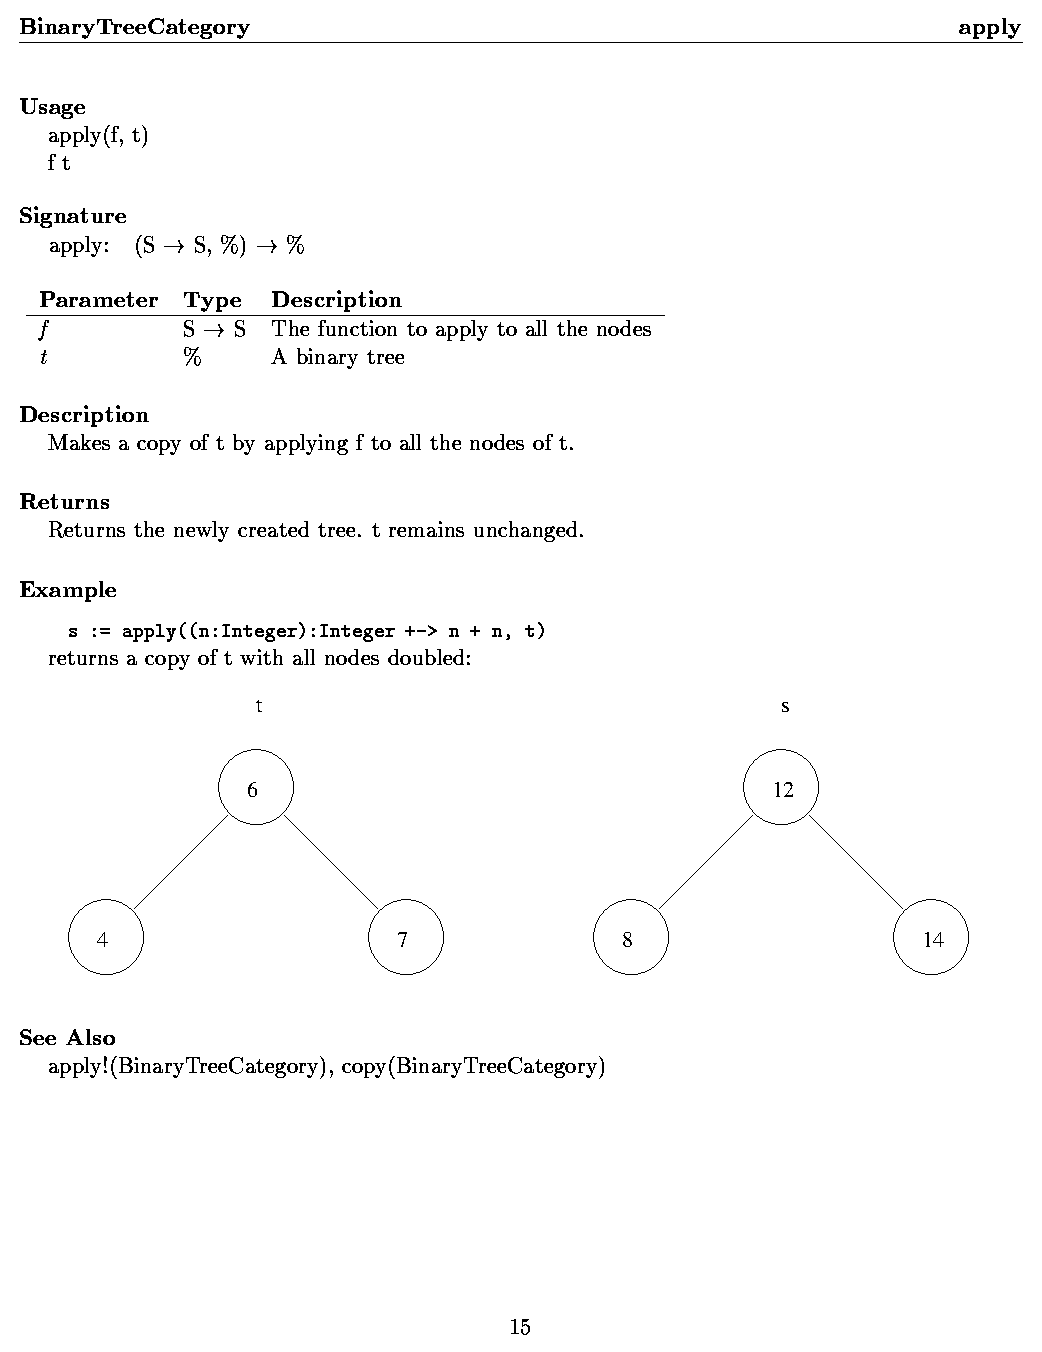
\epsfig{file=layout.eps, 
%    width=7cm}\hspace*{0.3cm}}\hfil
% \caption{manual page layout of the function \texttt{apply} belonging
%   to type \texttt{BinaryTreeCategory}}\label{fig:layout}
% \end{figure}
% 
% The \aldoc\ class file doesn't specify a manual page
% structure, except that types are described before their
% functions. However, we recommend using the description structure
% described below so that all \aldoc\ based manuals look similar.
%
% Types are like subsections and functions are subsubsections. Hence
% types are described first. If you don't follow this rule \aldoc\
% produces wrong index entries and some macros such as |\this| and
% |\name| return wrong results.
%
% The description of a type has the following structure:
%
% \pagebreak[2]
% \vspace{1ex}
% \hspace*{3ex}|\thistype[|\emph{short form}|]{|\emph{type name}|}| \newline
% \hspace*{6ex} [history section] \newline 
% \hspace*{6ex} [usage] \newline
% \hspace*{6ex} [parameters] \newline
% \hspace*{6ex} [description] \newline
% \hspace*{6ex} [exports] \newline
% \hspace*{6ex} [other sections] \newline
% 
% The \emph{history} section contains information about the author of
% the type, respectively function, as well as the date and nature of
% any changes made to the type or function. This piece of information
% is useful for software maintenance, especially when several
% programmers are working on the same library. However, this section
% is not printed in the final document unless you turn on a special
% flag.\footnote{The current version of \aldoc\ (v\fileversion) doesn't
% print the history section at all.}
%
% Functions belonging to a type are described in a similar way.
% 
% \vspace*{1ex}
% \hspace*{3ex}|\alpage{|\emph{function name}|}| \newline
% \hspace*{6ex} [history section] \newline
% \hspace*{6ex} [usage] \newline
% \hspace*{6ex} [signatures] \newline
% \hspace*{6ex} [parameters] \newline
% \hspace*{6ex} [description] \newline
% \hspace*{6ex} [return] \newline
% \hspace*{6ex} [example] \newline
% \hspace*{6ex} [see also] \newline
%
%
% \subsection{\aldoc\ macros in detail}
%
% \DescribeMacro{\thistype}
% |\thistype[|\emph{shortform}|]{|\emph{type}|}| starts the
% description of a type (called \emph{type}). The macro starts a new
% page and puts the type's name into the index, the table of contents
% and the header. The optional argument \emph{shortform} allows you to
% define a short form for the type's name.
%
% \docex{\cmd{thistype}\{Quotient\}}{} \\
% \docex{\cmd{thistype}[BinTree]\{BinaryTreeCategory\}}{} 
%
% The first example starts the description of the type
% \texttt{Quotient}, the latter of the type
% \texttt{BinaryTreeCategory} with the short form \texttt{BinTree}.
%
% \DescribeMacro{\this}
% \DescribeMacro{\shortthis}
% During the description of a type and its functions, the macros
% |\this| and |\shortthis| return the type's name and its abbreviated
% form. If no abbreviated form was given, then |\shortthis| returns the
% same result as |\this|. 
%
% \docex{\cmd{shortthis}\cmd{} is the short form for \cmd{this}.}{
%    BinTree is the short form for BinaryTreeCategory.}
%
% \DescribeMacro{\shortheader}
% Sometimes, type names are very long and use too much space in the
% header. Therefore, you might want to put a short form into the
% header. 
%
% The |\shortheader| command forces \aldoc\ to put the short
% form of the type into the header. If no short form was given then
% |\this| is put into the header.
%
% \docex{\cmd{thistype}[BinTree]\{BinaryTreeCategory\} \\
%   \cmd{shortheader}}{}
%
% \DescribeMacro{\alpage}
% The command |\alpage{|\emph{function}|}| starts the description of a
% new function (called \emph{function}). The macro clears the old page
% and puts the name of the function into the header and the index with
% the name of the type as a subentry. Note: the names of the functions
% are not added to the table of contents.  
%
% \docex{\cmd{alpage}\{apply\}}{}
%
% \DescribeMacro{\name}
% Similar to the |\this| command, the macro |\name| returns the name
% of the functions that is currently described. 
%
% \docex{\cmd{name}}{apply}
%
% Usually there are two versions of the \aldoc\ command. The first
% version, starting with a lowercase letter, is a \LaTeX\ environment,
% the second version, starting with an uppercase letter, is a \LaTeX\ 
% command. Both versions produce the same output.
%
% \vspace{1ex}
% |\begin{descr}              \Descr{Makes a copy of....}| \newline
% |   Makes a copy of....| \newline
% |\end{descr}|
% \vspace{1ex}
%
% Of course, the second version is faster to write, but if a long text
% has to be printed, then the environment version is easier to debug
% and uses less memory during \LaTeX\ compilation. 
% 
% \DescribeMacro{\History}
% The history section is not used by \aldoc\ yet. Nevertheless we
% encourage you to use the command already.
% 
% The |\History| command takes three arguments. Argument 1 contains
% the name of the author who created or changed the code. The date of
% the change is passed in argument 2 and comments are passed in
% argument 3. 
%
% \begin{quote} 
% \hspace*{-4ex}\texttt{\small{\cmd{History}\{A.~Einstein\}\{1912/3/13\}\{creation
% of the Relativity Theory\}}} \\
% \hspace*{-4ex}\texttt{\small{\cmd{History}\{G.~Lagaffe\}\{1995/2/28\}\{improved
% the theory\}}} \\
% \hspace*{-4ex}\texttt{\small{\cmd{History}\{G.~Lagaffe\}\{1995/3/1\}\{deleted 
% the improvements\}}}
% \end{quote}
%
% \DescribeEnv{usage}
% \DescribeMacro{\Usage}
% The usage part describes the usage of a function or a type, i.e.\
% how the function, respectively the type is called by the user. Both
% commands print the title \emph{Usage} in boldface and indent the
% left margin for the text that follows. 
%
% \docex{\cmd{Usage}\{apply(f,t)\}}{\textbf{Usage}
%    \begin{quote} apply(f,t) \end{quote}}
%
%
% \DescribeEnv{params}
% \DescribeMacro{\Params}
% Parameters are put in a tabular environment that is created
% automatically. The tabular contains three columns called
% \emph{Parameter}, \emph{Type} and \emph{Description} which are
% printed in boldface. The \& symbol is used as the column separator.
%
% \docex{\cmd{begin}\{params\} \\S \& Order \& The type of the node
%     $\backslash\backslash$ \\ 
%     t \& \cmd{\%} \& A binary tree $\backslash\backslash$\\
%     \cmd{end}\{params\}}{\hspace{-7ex}\begin{tabular}{lll}
%     \textbf{Parameter} & \textbf{Type} & \textbf{Description}\\ \hline
%     S & Order & The type of the nodes \\
%     t & \% & A binary tree \\
%     \end{tabular}}
%
% \DescribeEnv{descr}
% \DescribeMacro{\Descr}
% In the description section the type or function is described in
% detail. The  title \emph{Description} is printed in boldface and the
% left margin is indented for the text that follows. 
%
% \docex{\cmd{Descr}\{Makes a copy of t by applying f to all the nodes
%   of t.\}}{\textbf{Description}\begin{quote} Makes a copy of t by
%   applying f to all the nodes of t. \end{quote}} 
%
%
% \DescribeEnv{exports}
% The \emph{exports} section is only used for types. The environment
% creates a three column tabular. The first column contains the name
% of the exported function, the second column contains the signature
% of the function, and the last column contains notes describing the
% exported function. The export description of the type
% |BinaryTreeCategory| might look as follows: 
%
% \docex{\cmd{begin}\{exports\} \\
%   apply: \& (S \$\cmd{to}\$ S, \cmd{\%}) \$\cmd{to}\$ \cmd{\%} \&
%     Apply a function to all the nodes $\backslash\backslash$ \\
%     \$\cmd{ldots}\$ \& \& $\backslash\backslash$\\
%   \cmd{end}\{exports\}}{\hspace{-3ex}\textbf{Exports}
%     \begin{quote}\vspace*{-3ex}
%       \begin{tabular}{lll}
%          \hspace*{-7ex} apply: & (S $\to$ S, \%) $\to$ \% & Apply a
%          function \\
%          & & to all the nodes\\
%          \hspace{-7ex} $\ldots$ & & \\
%       \end{tabular}
%     \end{quote}}
%
% When types have arguments then the export list might depend
% on them, i.e.\ some functions are only exported if the
% argument has a specific category. Thus, the |exports| environment
% has an optional parameter that contains the condition under which the
% functions  are exported. The parameter immediately follows the
% |\begin{exports}| environment. 
% (|\begin{exports}[|\emph{condition}|]|) The following example shows
% a conditional export list (see also |example.as| on
% page~\pageref{example}):
%
% \docex{\cmd{begin}\{exports\}[if R has FiniteCharacteristic then]\\
% \cmd{category}\{FiniteCharacteristic\}$\backslash\backslash$ \\
% \$\cmd{ldots}\$ \& \& $\backslash\backslash$ \\
% \cmd{end}\{exports\}}{\hspace*{-3ex}\textbf{Exports}
%   \begin{quote}
%     \hspace*{-7ex}\mbox{if R has FiniteCharacteristic then} \\
%     \hspace*{-5ex}FiniteCharacteristic \\
%     \hspace*{-5ex}$\ldots$ \\
%   \end{quote}}
%   
% For each conditional export list an |exports| environment has to be
% used. 
%
% \DescribeMacro{hyperlinks}
% Imagine, you can click on types and functions in order to move to
% related topics? For example you look up a type or function in the
% index section, find the word and would like to click on it in order
% to jump to the corresponding page. Sounds like a web page. Well,
% formulas are not supported in html pages yet but we still can offer
% a similar way by using the \LaTeX\ package \texttt{hyperlink}. It offers
% link support for \texttt{xdvi}, pdf previewer and \LaTeXtoHTML. So with
% \texttt{xdvi} or Acrobat Reader\footnote{Acrobat Reader is a free
% pdf previewer from Adobe Systems Incorporated
% \texttt{http://www.adobe.com}} you are able to link pages. \aldoc\
% supports four commands for hyperlinks: |\alfunc|, |\alexp|,
% |\altype| and |\altarget|. We encourage to use this functions always,
% even if you don't plan to use hyperlinks. They can be turned on or
% off by a hyperlinks flag. See section \ref{hyperref}.
%
% \DescribeMacro{\alalias}
% With \aldoctohtml\, \aldor files, documented with \aldoc\ can be converted to HTML. 
% In order to support links in HTML documents \aldoc provides the command
% \cmd{alalias}\{\emph{type}\}\{\emph{alias}\}\{\emph{function}\}. It 
% creates a link to \emph{type:alias} and prints the name \emph{function}. 
% \cmd{alalias} is the basic command other commands relay on.
% 
% \DescribeMacro{\alfunc}
% \cmd{alfunc}\{\emph{type}\}\{\emph{function}\} prints \emph{function}
% and makes it a hyperlinks to the man page for \emph{function} in the
% type \emph{type}. The command is simply an abbreviation of 
% \cmd{alalias}\{\emph{type}\}\{\emph{function}\}\{\emph{function}\}.
%
% \docex{\cmd{begin}\{exports\} \\
%   \cmd{alfunc}\{Quotient\}\{apply\}: \& (S \$\cmd{to}\$ S, \cmd{\%}) \$\cmd{to}\$ \cmd{\%} \&
%     Apply a function to all the nodes $\backslash\backslash$ \\
%     \$\cmd{ldots}\$ \& \& $\backslash\backslash$\\
%   \cmd{end}\{exports\}}%  
%   {\hspace{-3ex}\textbf{Exports}
%     \begin{quote}\vspace*{-3ex}
%       \begin{tabular}{lll}
%          \hspace*{-7ex} apply: & (S $\to$ S, \%) $\to$ \% & Apply a
%          function \\
%          & & to all the nodes\\
%          \hspace{-7ex} $\ldots$ & & \\
%       \end{tabular}
%     \end{quote}}
%
% Note: the printed output does not differ from the output of the
% above example (|\exports|). If |hyperref| is turned on then links
% for |xdvi|, pdf previewers and of course in HTML are put into it.
%
% \DescribeMacro{\alexp}
% In the previous example you would have to write the type |Quotient| for
% each export field. You could also write
% \cmd{alfunc}\{\cmd{this}\}\{\emph{function}\} instead of the type name
% itself. \aldoc\ provides a shorthand for this command:
% \cmd{alexp}\{\emph{function}\} is the abbreviation of
% \cmd{alfunc}\{\cmd{this}\}\{\emph{function}\}.
%
% \DescribeMacro{\altype}
% \DescribeMacro{\altypes}
% Besides making links to functions, one likes to link to types
% as well. \aldoc\ offers the command \cmd{altype}\{\emph{type}\}
% for that purpose. It prints the name \emph{type} and makes it a
% hyperlinks to the manual page of that type, if defined.
% The command \cmd{altypes}\{\emph{header}\} puts the type name \emph{header}
% to the table of contents. This is usefull when types are grouped under 
% a name that should only appear in the table of contents.
%
% \docex{\cmd{begin}\{exports\} \\ \$\cmd{ldots}\$ \& \& $\backslash\backslash$\\
%   \cmd{alexp}\{order\}: \& (R,Integer) \$\cmd{to}\$
%   \cmd{altype}\{Partial\} \cmd{altype}\{Integer\} \&  
%   bounded ... $\backslash\backslash$ \\
%   \cmd{end}\{exports\}}{%
%   \hspace*{-7ex}\textbf{Exports}
%   \begin{quote}\vspace*{-2ex}
%     \begin{tabular}{lll}
%       \hspace*{-11ex} $\ldots$ & & \\
%       \hspace*{-11ex} order: & (R,Integer) $\to$ Partial Integer & bounded $\ldots$ \\ 
%       \hspace*{-11ex} $\ldots$ & & \\
%     \end{tabular}\\[0.3ex]
%   \end{quote}}
%
% \DescribeMacro{\albuiltin}
% \DescribeMacro{\alexttype}
% Both macros are used for external references. \cmd{albuiltin}\{\emph{type}\}
% is a reference to the builtin type \emph{type}, 
% \cmd{alexttype}\{\emph{library}\}\{\emph{type}\} is a reference of \emph{type}
% in the library \emph{library}.
%
% \docex{\cmd{albuiltin}\{Integer\} \\ \cmd{alexttype}\{Sumit\}\{Fraction\}}{}
%
% \DescribeMacro{\altarget}
% \cmd{altarget}|{|\emph{name}|}| creates an alternative hyper-target
% name. The command is useful when you have to link a page under
% several names. Example: If |\alpage{map}| documents both |map| and
% |map!|, then add the line |\altarget{map!}| right after it. This
% way, if both |\alexp{map}| and |\alexp{map!}| are in the exports
% list, they will both point to that page.
%
% \DescribeMacro{\category}
% Sometimes types export categories. Of course, you could write the
% category's name in the first column, but usually the names are very
% long and, thus, enlarge the first column of the tabular in such a way
% that the output looks ugly. To overcome this problem the macro
% |\category| is introduced. It takes a name as argument and prints it
% on one line, i.e.\ three columns are combined to one column. In
% fact, |\category| is an abbreviation for |\multicolumn{3}{l}|.  
%
% \docex{\cmd{begin}\{exports\} \\ \$\cmd{ldots}\$ \& \& $\backslash\backslash$\\
%   \cmd{category}\{\cmd{altype}\{CommutativeRing\}\} $\backslash\backslash$ \\
%   \$\cmd{ldots}\$ \& \& $\backslash\backslash$ \\ 
%   \cmd{end}\{exports\}}{\textbf{Exports}
%   \begin{quote}
%     $\ldots$ \\
%     CommutativeRing \\
%     $\ldots$ \\
%   \end{quote}}
%
% \DescribeEnv{alwhere}
% If names in export tabulars are too long, then one might whish to
% abbreviate the name and explain it in detail below the tabular. 
% Therefore, \aldoc\ contains the environment |alwhere| which usually
% follows after an \emph{export} environment. It prints the name
% \emph{where} and creates a three column tabular.
%
% \docex{\cmd{begin}\{exports\} \\ \$\cmd{ldots}\$ \& \& $\backslash\backslash$\\
%   order: \& (R,Z) \$\cmd{to}\$ Partial Z \& 
%   bounded order at the place $\backslash\backslash$ \\
%   \cmd{end}\{exports\}\\
%   \cmd{begin}\{alwhere\} \\
%   Z \& == \& \cmd{altype}\{Integer\} $\backslash\backslash$ \\
%   \$\cmd{ldots}\$ \& \& $\backslash\backslash$ \\
%   \cmd{end}\{alwhere\}}{\hspace*{-7ex}\textbf{Exports}
%   \begin{quote}\vspace*{-2ex}
%     \begin{tabular}{lll}
%       \hspace*{-11ex} $\ldots$ & & \\
%       \hspace*{-11ex} order: & (R,Z) $\to$ Partial Z & bounded order at place \\
%       \hspace*{-11ex} $\ldots$ & & \\
%     \end{tabular}\\[0.3ex]
%     \hspace*{-10ex}where \\
%     \begin{tabular}{lcl}
%       \hspace*{-10ex}Z & == & Integer \\
%       \hspace*{-10ex}$\ldots$ & & \\
%     \end{tabular}
%   \end{quote}}
%
% \DescribeEnv{signatures}
% \DescribeMacro{\Signatures}
% A signature describes the types of the arguments and the type of the
% return value. Obviously a signature only makes sense to functions
% and, hence, you will never use such a command in a type description.
% The title \emph{Signatures} is printed in boldface and
% the left margin is indented. Both commands open a tabular environment
% with two columns (function's name, signature).
%
% \docex{\cmd{begin}\{signatures\}\\apply: \& (S \$\cmd{to}\$ S, \%)
% \$\cmd{to}\$ \cmd{\%} 
%      $\backslash\backslash$ \\ \cmd{end}\{signatures\}}{\textbf{Signatures}
%      \begin{quote}
%      \begin{tabular}{ll}
%        apply: & (S $\to$ S, \%) $\to$ \% \\
%      \end{tabular}
%      \end{quote}}
%
% \DescribeMacro{\Signature}
% Often only one signature has to be printed. Therefore, \aldoc\ has a
% special signature command called |\Signature|. It prints the title
% \emph{Signature} and indents the left margin. Unlike the
% commands |\Signatures| and |signatures|, |\Signature| prints
% the name of the function automatically. Hence, the macro has only
% two  arguments, the parameter signature (argument 1) and the return
% type signature (argument 2). The signature is printed in the
% following way: \emph{name~of~the~function}:~\#1~$\to$~\#2 where \#1
% is the first argument and \#2 the second.
%
% \docex{\cmd{signature}\{(S \$\cmd{to}\$ S,
%     \cmd{\%})\}\{\cmd{\%}\}}{\textbf{Signature} 
%     \begin{quote} 
%     \begin{tabular}{ll}
%       apply: & (S $\to$ S, \%) $\to$ \% \\
%     \end{tabular}
%     \end{quote}}
%
% \DescribeMacro{\alconstant}
%  Sometimes a constant is defined only. The command
% \cmd{alconstant}\{\emph{type}\} prints the function name implicitly and puts
% the type of the constant to the right. 
% \docex{\cmd{alconstant}\{\cmd{albuiltin}\{SingleFloat\}\}}%
%    {\textbf{Signature}
%    \begin{quote}
%       \begin{tabular}{ll}
%          PI: & SingleFloat \\
%       \end{tabular}
%    \end{quote}}
%
% \DescribeEnv{retval}
% \DescribeMacro{\Retval}
% This describes the return value of a function. Again, the title
% \emph{Returns} is printed in boldface and the left margin indented 
% for the text that follows. 
%
% \docex{\cmd{begin}\{retval\} \\ 
%    Returns the newly created tree. \\ t remains unchanged. \\ 
%    \cmd{end}\{retval\}}{\textbf{Returns}
%     \begin{quote} Returns the newly created tree. t remains
%     unchanged.\end{quote}}
%
% \DescribeEnv{alex}
% It's sometimes useful to add examples in a manual page. Therefore,
% \aldoc\ supports the command |\alex|. The command prints
% the title \emph{Example} in  boldface and indent the left margin. 
%
% \docex{\cmd{begin}\{alex\}\\ 
%    \cmd{begin}\{ttyout\} \\
%    s:=~apply((n:Integer):Integer~+->~n+n,~t)
%    \cmd{end}\{ttyout\} \\
%    returns a copy of t with all nodes doubled. \\
%    \cmd{end}\{alex\}}{\textbf{Example}\begin{quote}
%    \vspace{-3ex}
%    \hspace*{-3ex}\texttt{s:=~apply((n:Integer):Integer~+->~n+n,~t)} \\
%    \hspace*{-3ex}\mbox{returns a copy of t with all nodes doubled.}
%    \end{quote}}
%
% In example sections, you often use the verbatim environment for
% source code or output produced by the system. \aldoc\ doesn't have
% its own verbatim macros, but it includes the verbatim package
% \texttt{ttyverb}\footnote{Note: \texttt{ttyverb} is the name of the
% package and \texttt{ttyout} is the name of the environment
% defined in \texttt{ttyverb}.} which has the following advantages over the
% original verbatim package included in \LaTeX:  
% \begin{itemize}
%   \item font and size can by changed,
%   \item the vertical space is narrower than the \LaTeX\ version of
%     verbatim 
%   \item tabs are converted to as many spaces as you like (default 8)
% \end{itemize}
%
% Of course, you can use your own verbatim macros, but using
% \texttt{ttyverb} makes life easier when you distribute documented
% \aldor\ code to other people. A detailed description of
% \texttt{ttyverb} is found in the \texttt{ttyverb.sty} style file.
% 
% \DescribeMacro{\alseealso}
% Often one would like to give references to other functions or types 
% containing useful information. Therefore \aldoc\ contains the
% |\alseealso| command that takes the references as argument. 
%
% \docex{\cmd{alseealso}\{\cmd{alexp}\{apply!\}\}}{\textbf{See Also}
%     \begin{quote} apply! \end{quote}}
%
% Note: \cmd{alseealso} is also a place where one likes to have hyper
% references, ie.\ links to the mentioned functions.
%
% \DescribeEnv{remarks}
% \DescribeMacro{\Remarks}
% Sometimes you want to add remarks to a manual page. It's especially
% useful when limitations in the use of a function or type or bugs
% that are not fixed yet. The commands |remarks|, |\Remarks| print the
% title \emph{Remarks} in  boldface and indent the left margin. 
%
% \docex{\cmd{Remarks}\{\cmd{this}$\backslash$ still crashes when
%   \$\cmd{ldots}\$}{\textbf{Remarks}
%     \begin{quote} BinaryTree still crashes when $\ldots$ \end{quote}}
%
% \subsection{A word about Hyper-References}\label{hyperref}
%
% We strongly recommend to use the hyper-reference features provided
% in \aldoc, ie.\ \cmd{alfunc}, \cmd{alexp}, \cmd{altype}, \cmd{albuiltin}, 
% \cmd{alexttype} and \cmd{altarget}. Even when the \texttt{hyperref} 
% package is not installed on your system or you do not want to use 
% \LaTeXtoHTML\ yet, you can produces printed output without any problems. By
% default hyper-reference is turned off and the hyper-reference
% commands produces the usual output. To turn on hyper-reference you
% have to set the \emph{hyperref} option in the latex file. 
%
% \docex{%
% \cmd{documentclass}[hyperref]\{aldoc\}}{will turn on hyper-reference}
%
% \subsection{Putting everything together}
%
% In the previous sections we explained the \aldoc\ macros in detail
% but said nothing about \aldor\ files. Before you can create the
% \TeX\ files using the \extract\ utility, you must be sure that all
% documentation lines in your source files are bracketed between
% |#if|~\emph{marker} and |#endif| statements where \emph{marker} can
% by any name. \extract\ takes as input a \aldor\ file and the
% \emph{marker} and produces the \LaTeX\ file by discarding the code
% that is not between |#if|~\emph{marker} and |#endif| statements. In
% each \aldor\ source file you must add the |#unassert|~\emph{marker}
% statement before the first |#if|~\emph{marker} statement starts.
%
% The \sumit\ library for which this class file originally was written
% uses |ASDOC| as its marker, \salli\ uses |ALDOC| as its marker. We
% encourage you to use the same marker depending on the library you
% are working with, because whenever |sumit.as| or |aldor.as| is
% included, |ASDOC|, |ALDOC| respectively is already unasserted and
% hence, the |#unassert ASDOC| or |#unassert ALDOC| statement can be
% omitted. 
%
% |#unassert ALDOC   % can be omitted if you include aldor.as| \\
% |...| \\
% |#if ALDOC| \\
% |This is some documentation which will be ignored by | \\
% |the A# compiler.| \\
% |...| \\
% |#endif| \\
% |[A# code]| \\
% |#if ALDOC| \\
% |This is again documentation.| \\
% |#endif| \\
% |[A# code again]| \\
%
% In the documentation parts, i.e.\ between |#if|~\emph{marker} and |#endif|
% statements, you can use any \aldoc\ or \LaTeX\ command.
%
%
% \subsection{\extract\ option}
%
% The general usage of \extract\ is:
% \begin{center}
% \extract\ -m \emph{marker} [-h] [-o \emph{outputfile}] [-r] [-t] [-v]
% \emph{sourcefile}[.as]
% \end{center}
% where the various options are:
% 
% \begin{itemize}
% \item[-h] Help: displays a short help text (causes all the other
%   arguments to be ignored).
% \item[-m] \emph{marker} Defined marker in the
%   \emph{sourcefile}. Note: No default value is defined.
% \item[-o] \emph{outputfile} Names the output file, default is
%   \emph{sourcefile.tex} 
% \item[-r] Reverse operation: the output file contains all the lines
%   which are not bracketed between |#if|~\emph{marker} and |#endif|
%   statements. 
% \item[-t] Test: adds an appropriate \LaTeX\ prologue and epilogue
%   so that the output file can be run through \LaTeX\
%   independently.
% \item[-v] Verbose: shows progress (number of documentation blocks
%   processed.) 
% \end{itemize}
%
%
% \subsection{The manual \LaTeX\ file}
%
% When your \aldor\ programs are documented and \extract\ has created
% the \LaTeX\ files then you are ready to write the final ``manual''
% file. This \LaTeX\ file turns some \aldoc\ features on or off and
% contains text you want to add to the manual pages. A ``manual''
% file might look like this:
%
% \begin{quote}
% |\documentclass[|\emph{options}|]{aldoc}| \\
% \emph{packages} \\
% |\pagestyle{fancyhdr}      % header creation turned on |  \\
% |\makeindex                % create index| \\
% |\begin{document}| \\
% \emph{introduction, table of contents, table of figures and so on} \\
% |\input{...}| \\
% \emph{other imports} \\
% |\printindex               % print index| \\
% |\end{document}| \\
% \end{quote}
%
% \emph{options} can be any valid option under \LaTeX\ such as
% twoside, 12pt, a4paper and so on. If you want to use the
% hyper-reference features from \aldoc\ then you have to set the
% \texttt{hyperref} option! In the \emph{packages} part you can
% include additional packages that are used in your document. However,
% the packages \texttt{fancyhdr}, \texttt{epsfig},
% \texttt{supertabular}, \texttt{ttyverb} and \texttt{makeidx} don't
% have to be loaded because \aldoc\ loads them automatically. 
%
% If you want to print your document using the standard \aldoc\ header
% then you have to call pagestyle with fancyplain. If you omit this
% command then no header is printed. An index is created by \LaTeX\
% when \texttt{makeindex} is called in the preamble. If you comment out
% the command no index is generated. 
% A detailed description of the \texttt{makeindex} and the
% \texttt{fancyhdr} packages is found in~\cite{gms:latexComp}.   
%
% One last thing you have to keep in mind is that the command
% |\thistype| is the same as a subsection but without a subsection
% number. Of course, you can create sections and subsections, but the
% latter does not get a subsection number. 
%
%
% \subsection{Aldoc2HTML}
% 
% Version~3 of \aldoc\ has better html support. The utility \aldoctohtml\
% converts |.tex| files created with the \extract\ utility to new |.tex|
% files which are optimized for the \LaTeXtoHTML\ utility.
%
% The general usage of \aldoctohtml\ is:
% \begin{center}
% \aldoctohtml\ [-h] [-o \emph{outputfile}] [-x] [-v]
% \emph{sourcefile}[.tex]
% \end{center}
% where the various options are:
% 
% \begin{itemize}
% \item[-h] Help: displays a short help text (causes all the other
%   arguments to be ignored).
% \item[-o] \emph{outputfile} Names the output file, default is
%   standard output. 
% \item[-x] Input: expands only \cmd{input} statements.
% \item[-v] Verbose: shows progress. 
% \end{itemize}
%
% In order to create a HTML version of the documentation do the following:
% \begin{enumerate}
% \item Create \aldor\ source files documentend with the \aldoc\ style file.
% \item Extract the documentation |.tex| by using the \extract\ utility.
% \item Create HTML optimized \LaTeX\ files by using the \aldoctohtml\ utility.
% \item Run \LaTeXtoHTML\ to create the HTML files.
% \end{enumerate}
%
%
% \subsection{Example}
%
% In this section we create the manual pages of the
% |example.as| file. The described type is called |Quotient|. The
% following code fragment shows the documented \aldor\ file. Note:
% |example.as| is shipped with this package but it cannot be compiled
% with \aldor\ because it contains a category not provided by the
% standard library. However, it can be used as a template for your own
% documentation (|extract| can create the \LaTeX\ file, which can then be
% processed).
%
% \label{example}
% \vspace{1ex}
% |#include "aldor.as"| \\
% |#unassert ALDOC| \\
% || \\
% |#if ALDOC| \\
% || \\
% |\thistype{Quotient}| \\
% |\History{G.~Lagaffe}{1/12/94}{created}| \\
% || \\
% |\Usage{import from \this~R}| \\
% || \\
% |\Params{ \emph{R} & \altype{IntegralDomain} | \\
% |        & an integral domain\\ | \\
% |}| \\
% || \\
% |\Descr{\this~R forms the quotient field of the | \\
% |integral domain \emph{R}}| \\
% || \\
% |\begin{exports}| \\
% |\category{\altype{Field}}\\| \\
% |\category{\altype{DifferentialExtension} R}\\| \\
% |$/$: & (R,R) $\to$ \% & take the quotient of two | \\
% |ring elements\\| \\
% |\alexp{coerce}: & R $\to$ \% & coercion from R to \this\\| \\
% |\alexp{denominator}: & \% $\to$ R & get the denominator of a quotient\\| \\
% |\alexp{numerator}: & \% $\to$ R & get the numerator of a quotient\\| \\
% |\end{exports}| \\
% |\begin{exports}[if R has \altype{FiniteCharacteristic} then]| \\
% |\category{\altype{FiniteCharacteristic}}\\| \\
% |\end{exports}| \\
% |\begin{exports}[if R has \altype{GcdDomain} then]| \\
% |\alexp{normalize}: & \% $\to$ \% & normalize a quotient\\| \\
% |\end{exports}| \\
% |#endif| \\
% || \\
% |Quotient(R: IntegralDomain):| \\
% | Join(Field, DifferentialExtension R) with {| \\
% |     /:      (R, R) -> %;| \\
% || \\
% |#if ALDOC| \\
% |\alpage{/}| \\
% || \\
% |\Usage{n~\name~d}| \\
% |\Signature{(R,R)}{\%}| \\
% |\Params{| \\
% |\emph{n} & R & An element of the ring.\\| \\
% |\emph{d} & R & An element of the ring.\\| \\
% |}| \\
% |\Retval{Returns the quotient \emph{n} over \emph{d}.}| \\
% |#endif| \\
% || \\
% |     if R has FiniteCharacteristic then | \\
% |         FiniteCharacteristic;| \\
% |     coerce:     R -> %;| \\
% | | \\
% |#if ALDOC| \\
% |\alpage{coerce}| \\
% || \\
% |\Usage{\name~x}| \\
% |\Signature{R}{\%}| \\
% |\Params{ \emph{x} & R & An element of the ring\\ }| \\
% |\Retval{Returns the quotient with numerator \emph{x} and | \\
% |        denominator 1.| \\
% |}| \\
% |#endif| \\
% || \\
% |     denominator:    % -> R;| \\
% | | \\
% |#if ALDOC| \\
% |\alpage{denominator}| \\
% || \\
% |\Usage{\name~x}| \\
% |\Signature{\%}{R}| \\
% |\Params{ \emph{x} & \% & A quotient\\ }| \\
% |\Retval{Returns the denominator of a quotient.}| \\
% |\alseealso{\alexp{numerator}| \\
% |#endif| \\
% || \\
% |     if R has GcdDomain then| \\
% |         normalize:  % -> %;| \\
% |     | \\
% |#if ALDOC| \\
% |\alpage{normalize}| \\
% |\Usage{\name~x}| \\
% |\Signature{\%}{\%}| \\
% |\Params{ \emph{x} & \% & An quotient\\ }| \\
% |\Descr{Normalize $x$ by eliminating common divisors of | \\
% |       the numerator and denominator.| \\
% |}| \\
% |#endif| \\
% || \\
% |     numerator:  % -> R;| \\
% | | \\
% |#if ALDOC| \\
% |\alpage{numerator}| \\
% || \\
% |\Usage{\name~x}| \\
% |\Signature{\%}{R}| \\
% |\Params{ \emph{x} & \% & A quotient\\ }| \\
% |\Retval{Returns the numerator of a quotient.}| \\
% |\alseealso{\alexp{denominator}}| \\
% |#endif| \\
% |} == add {| \emph{implementation} |}| \\
%
% First we produce the corresponding \LaTeX\ file by using the
% \extract\ utility. 
%
% \hspace*{2ex}|extract -m ALDOC example.as|
%
% The extract utility creates the file |example.tex|. Now we
% have to create the ``manual'' \LaTeX\ file that looks as follows: 
%
% \vspace{1ex}
% |% manual.tex|\\
% |\documentclass[12pt,hyperref]{aldoc}|\\
% |\pagestyle{fancyplain}|\\
% |\makeindex|\\
% |\begin{document}|\\
% |\thistype{Quotient}
\History{L.~Lagaffe}{1/12/94}{created}

\Usage{import from \this~R}

\Params{ \emph{R} & IntegralDomain 
        & an integral domain\\ 
}

\Descr{\this~R forms the quotient field of the 
integral domain \emph{R}}

\begin{exports}
\category{\astype{Field}}\\
\category{\astype{DifferentialExtension} R}\\
$/$: & (R,R) $\to$ \this & take the quotient of two 
ring elements\\
\asexp{coerce}: & R $\to$ \% & coercion from R to \this\\
\asexp{denominator}: & \% $\to$ R & get the denominator of a quotient\\
\asexp{numerator}: & \% $\to$ R & get the numerator of a quotient\\
\end{exports}
\begin{exports}[if R has \astype{FiniteCharacteristic} then]
\category{\astype{FiniteCharacteristic}}\\
\end{exports}
\begin{exports}[if R has \astype{GcdDomain} then]
\asexp{normalize}: & \% $\to$ \% & normalize a quotient\\
\end{exports}
\aspage{/}

\Usage{n~\name~d}
\Signature{(R,R)}{\%}
\Params{
\emph{n} & R & An element of the ring.\\
\emph{d} & R & An element of the ring.\\
}
\Retval{Returns the quotient \emph{n} over \emph{d}.}
\aspage{coerce}

\Usage{\name~x}
\Signature{R}{\%}
\Params{ \emph{x} & R & An element of the ring\\ }
\Retval{Returns the quotient with numerator \emph{x} and 
        denominator 1.
}
\aspage{denominator}

\Usage{\name~x}
\Signature{\%}{R}
\Params{ \emph{x} & \% & A quotient\\ }
\Retval{Returns the denominator of a quotient.}
\seealso{\astype{numerator}(\this)}
\aspage{normalize}
\Usage{\name~x}
\Signature{\%}{\%}
\Params{ \emph{x} & \% & An quotient\\ }
\Descr{Normalize $x$ by eliminating common divisors of 
       the numerator and denominator.
}
\aspage{numerator}                                                  

\Usage{\name~x}
\Signature{\%}{R}
\Params{ \emph{x} & \% & A quotient\\ }
\Retval{Returns the numerator of a quotient.}
\seealso{\astype{denominator}(\this)}
|\\
% |\printindex|\\
% |\end{document}|\\
%
% In the last step we have to compile |manual.tex|, create the index
% with \texttt{makeindex} and compile the manual again. 
%
% \vspace{1ex}
% |latex manual.tex|\\
% |makeindex manual.idx|\\
% |latex manual.tex| \\
%
% Figure~\ref{fig:manual} and figure~\ref{fig:manualB} show 
% the manual pages produced.
%
%
% \begin{figure}
% \mbox{
% \fbox{\hspace*{1ex}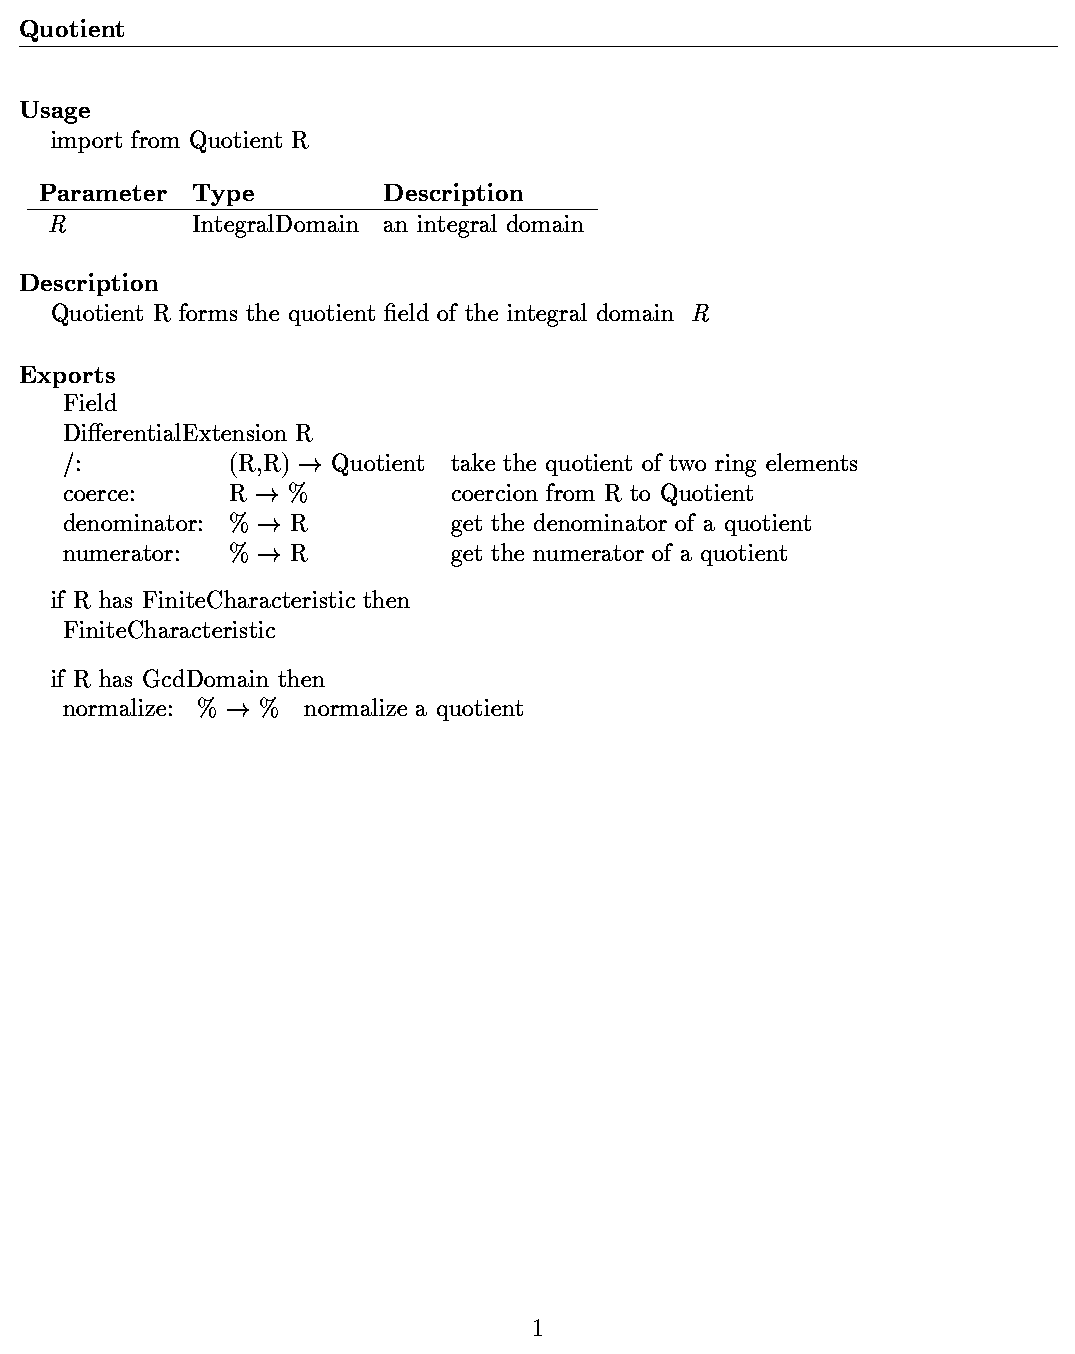
\epsfig{file=page1.eps, width=6cm}\hspace*{1ex}} 
% \hspace{1ex}
% \fbox{\hspace*{1ex}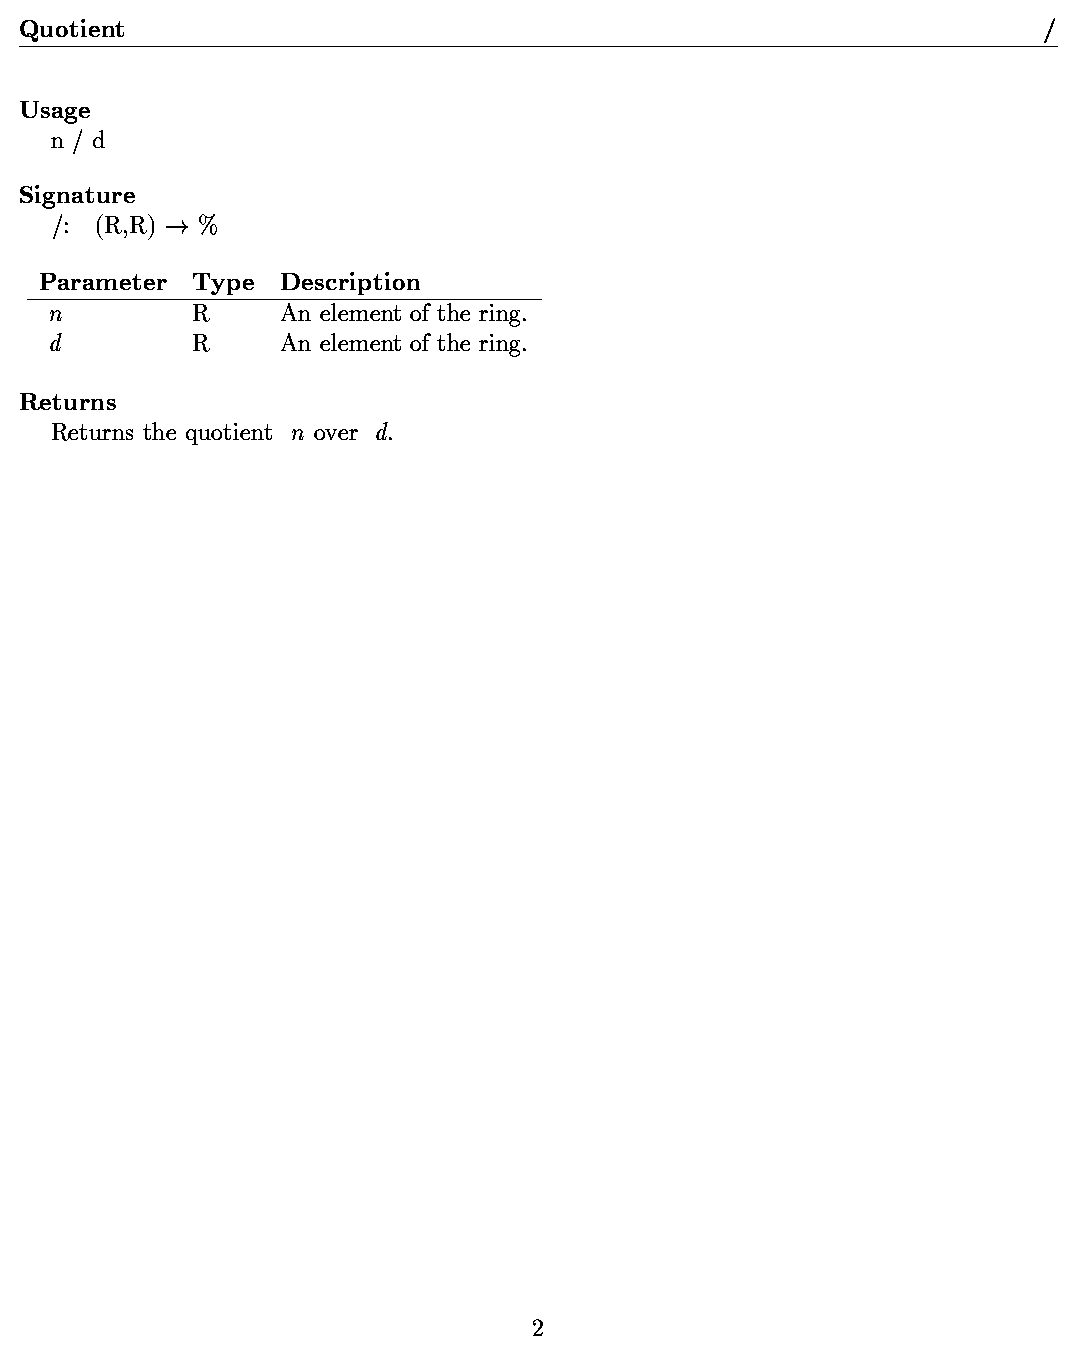
\epsfig{file=page2.eps, width=6cm}\hspace*{1ex}}
% }
%
% \vspace{1ex}
% \mbox{
% \fbox{\hspace*{1ex}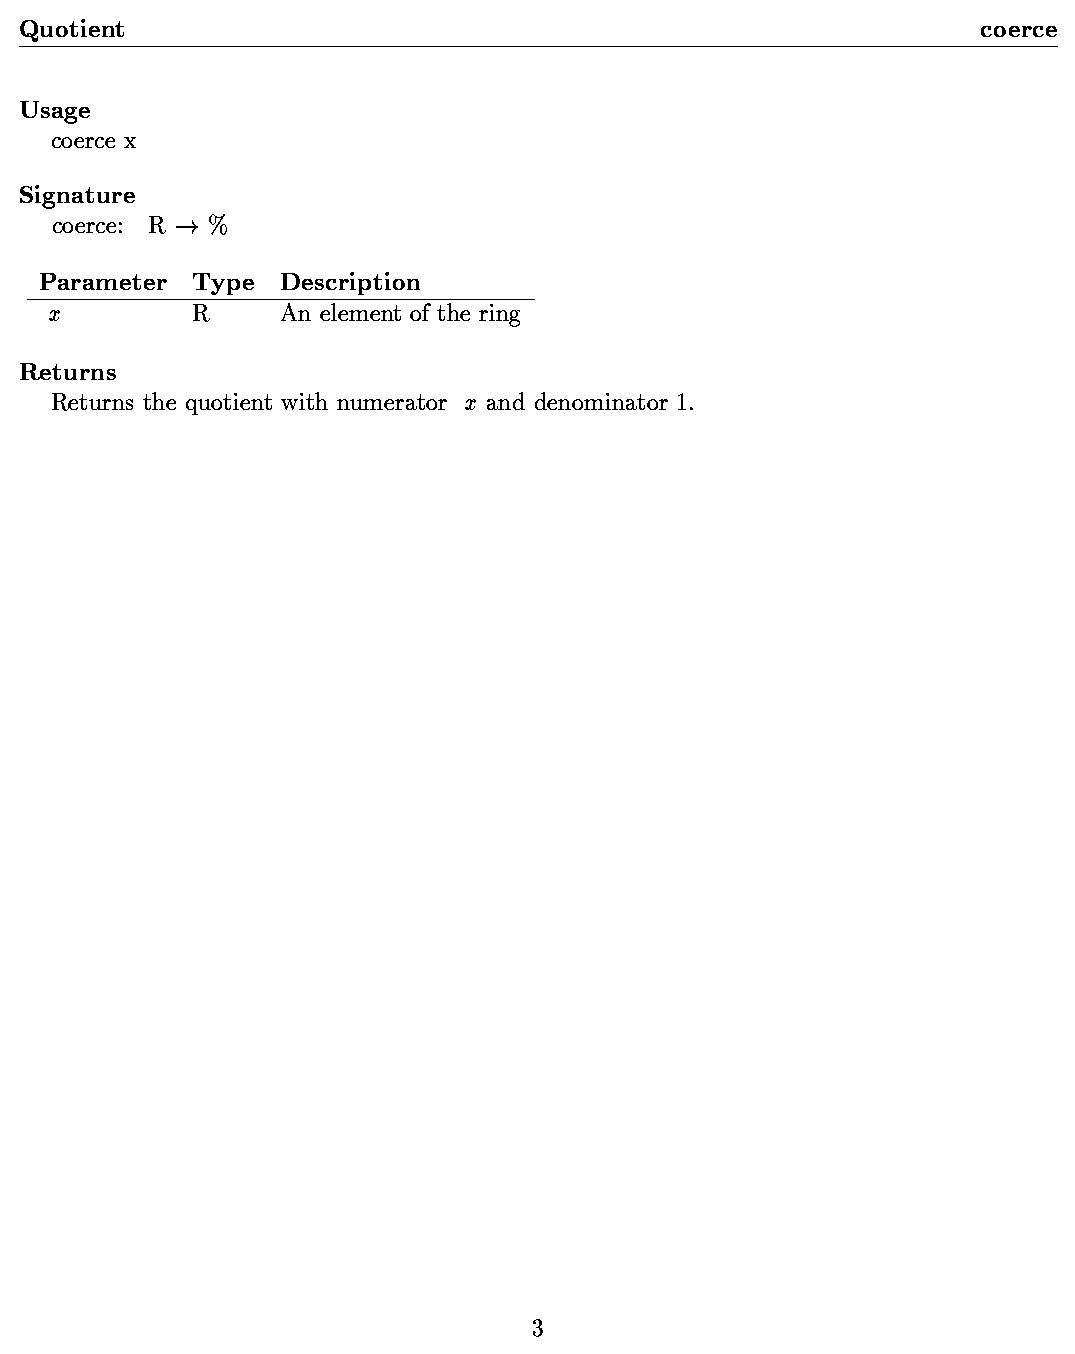
\epsfig{file=page3.eps, width=6cm}\hspace*{1ex}}
% \hspace{1ex}
% \fbox{\hspace*{1ex}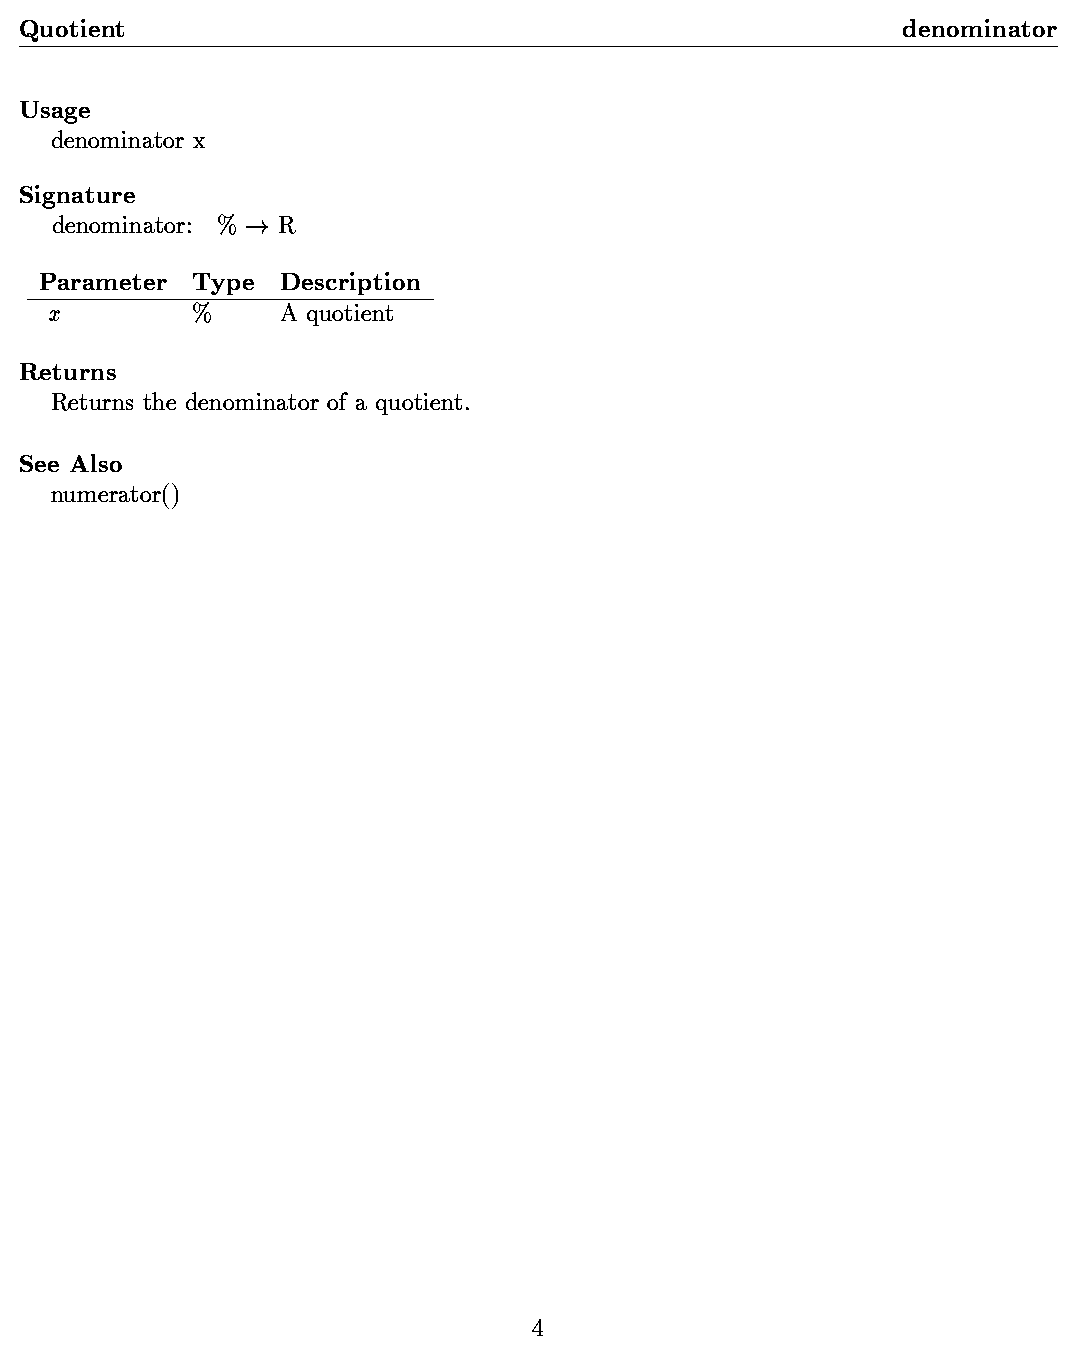
\epsfig{file=page4.eps, width=6cm}\hspace*{1ex}}
% }
% \caption{Manual pages from ``manual.tex''.}\label{fig:manual}
% \end{figure}
%
% \begin{figure}
% \mbox{
% \fbox{\hspace*{1ex}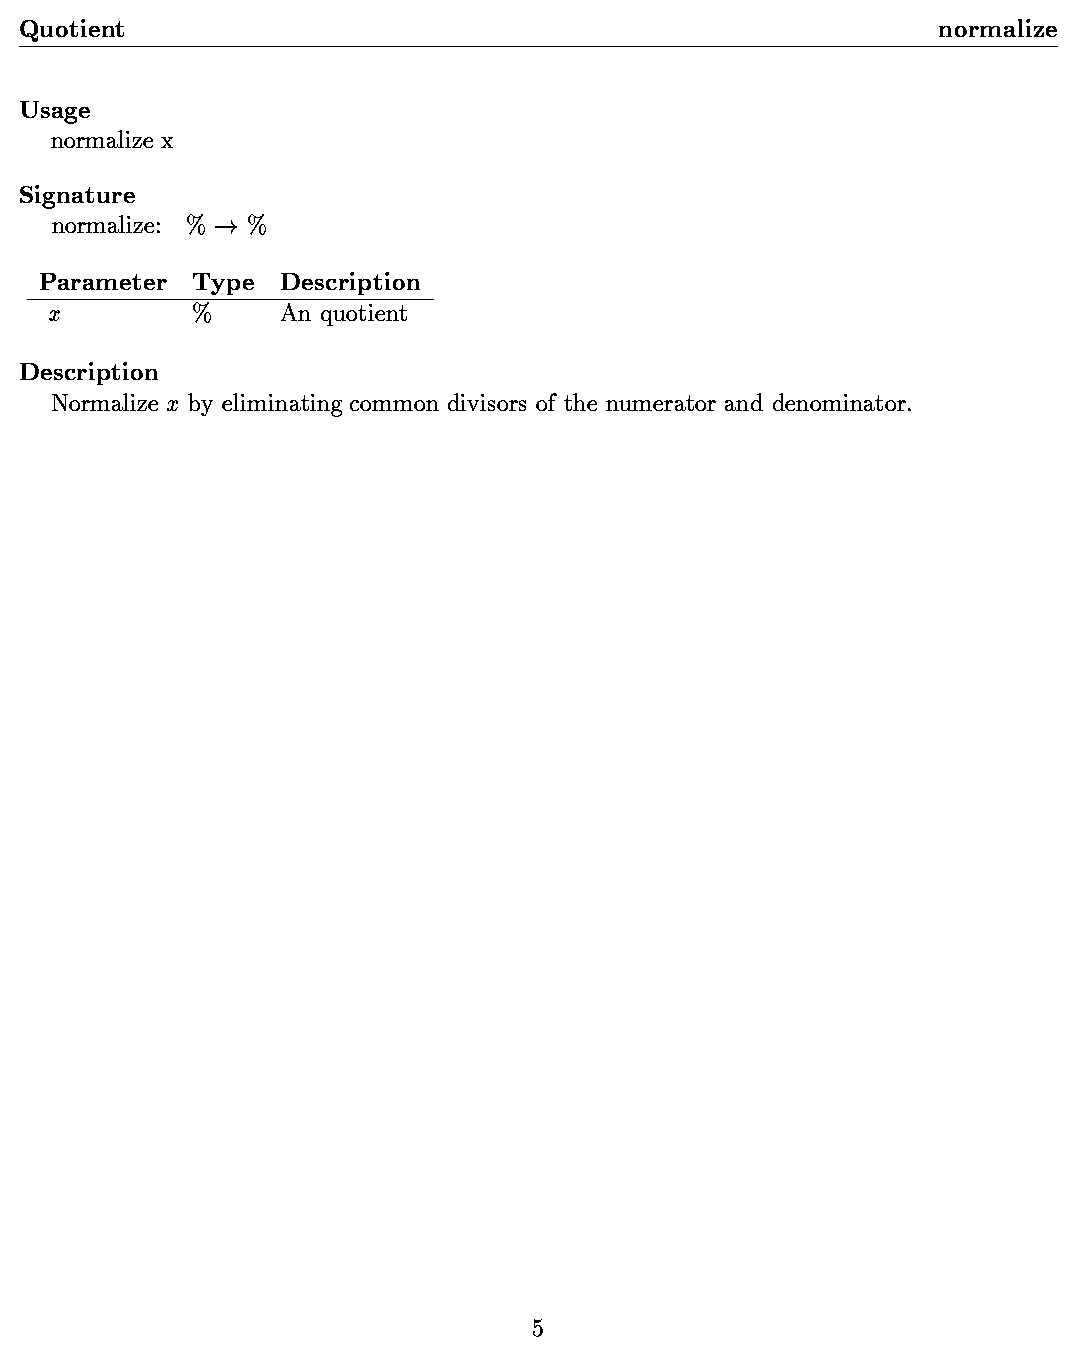
\epsfig{file=page5.eps, width=6cm}\hspace*{1ex}} 
% \hspace{1ex}
% \fbox{\hspace*{1ex}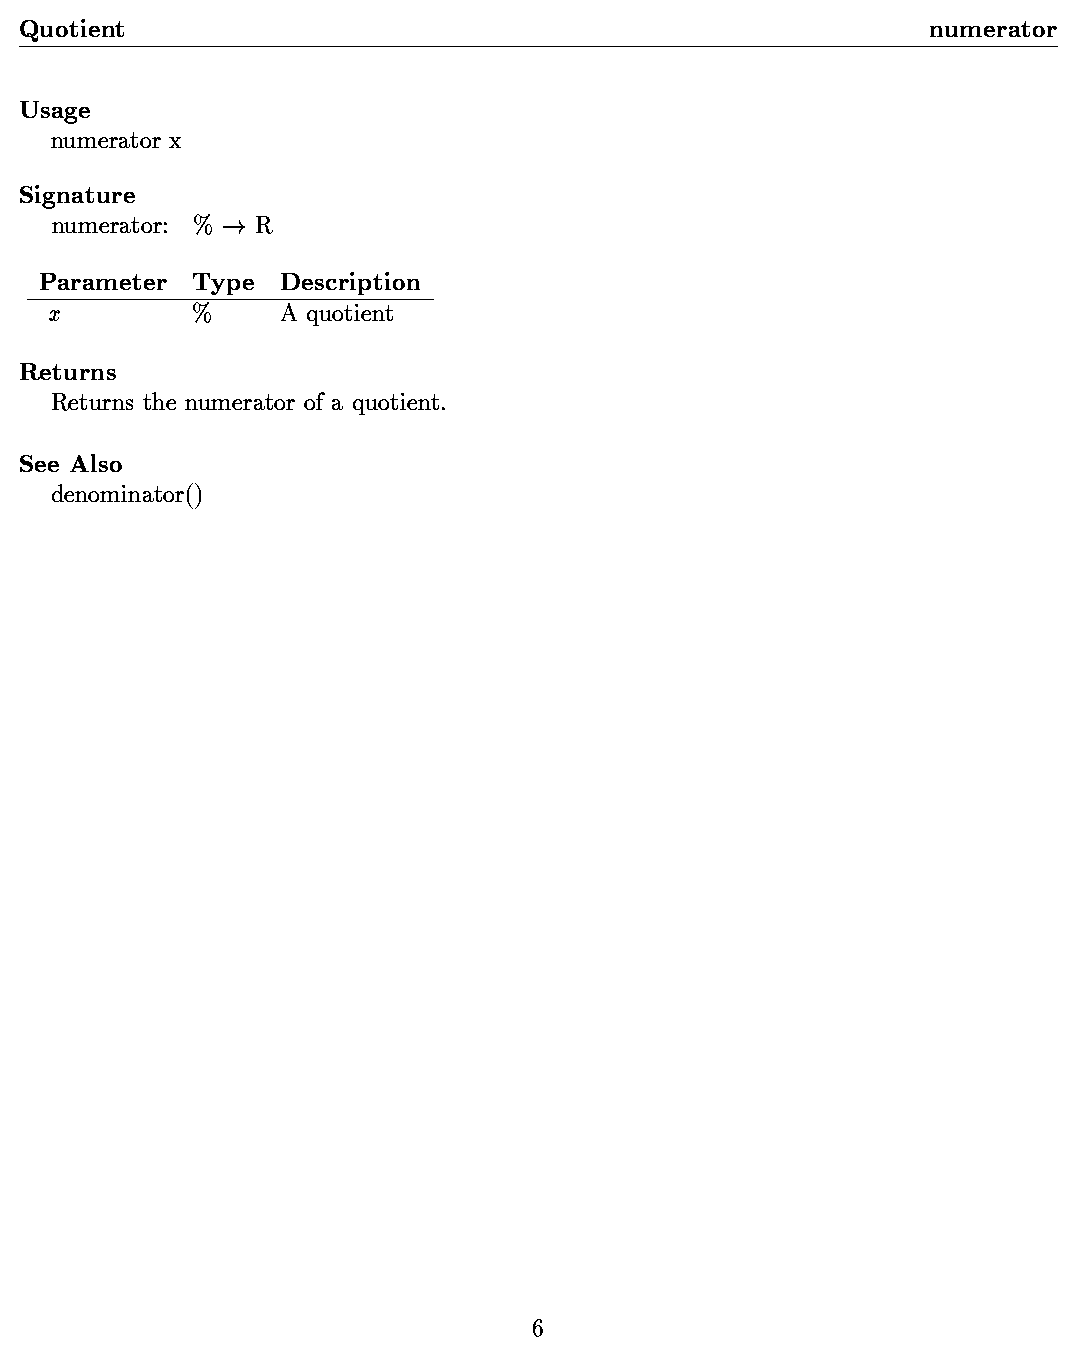
\epsfig{file=page6.eps, width=6cm}\hspace*{1ex}}
% }
%
% \vspace{1ex}
% \mbox{
% \fbox{\hspace*{1ex}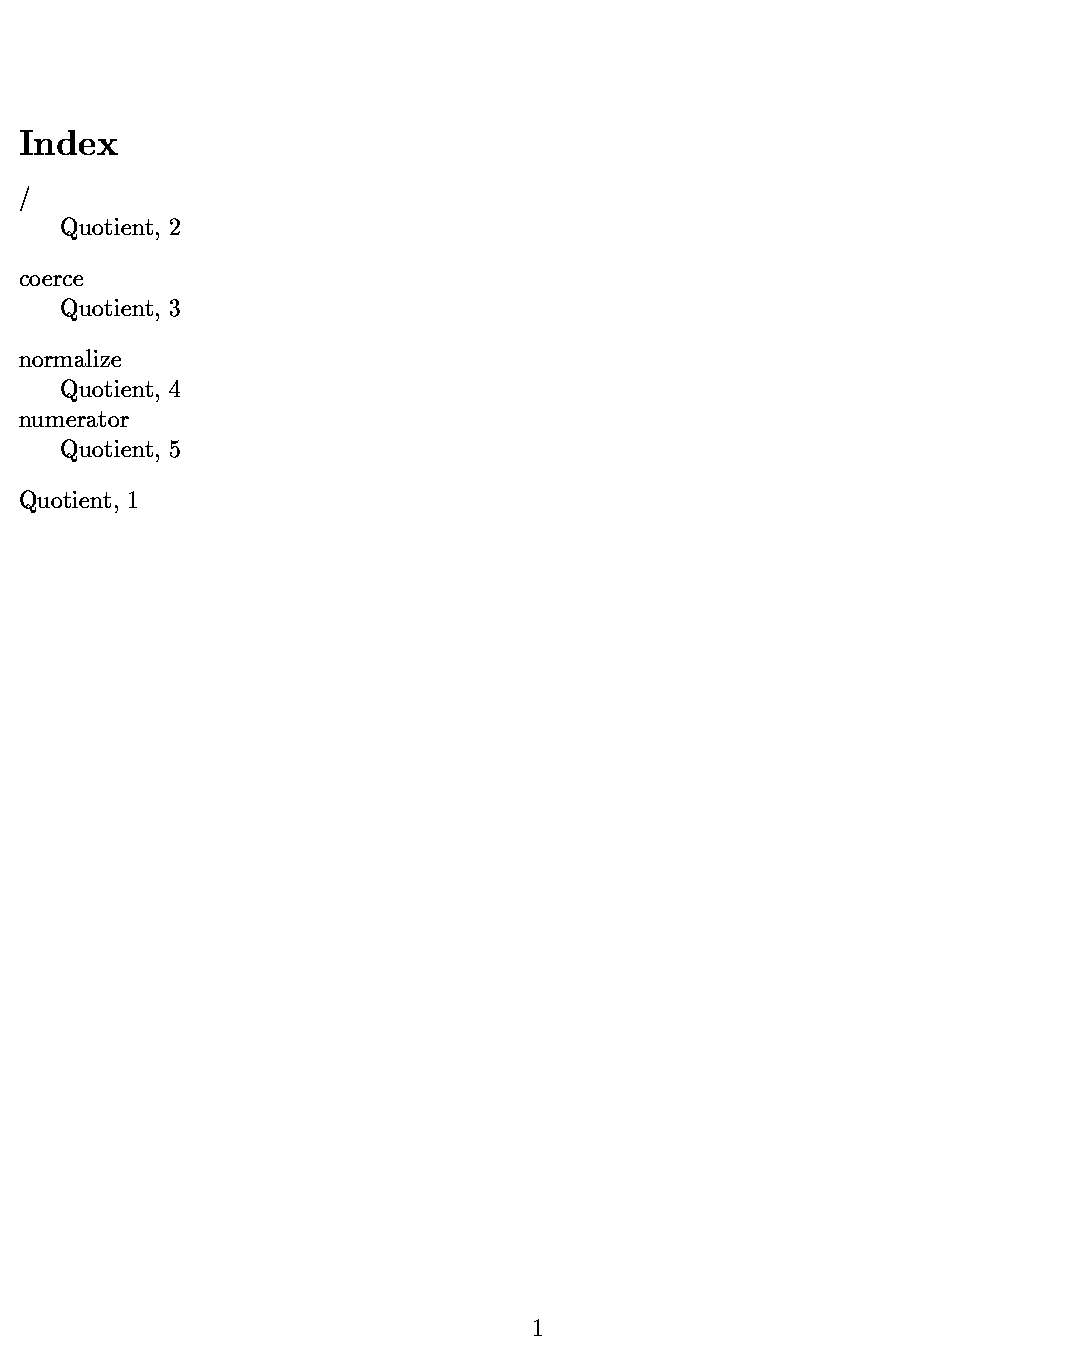
\epsfig{file=page7.eps, width=6cm}\hspace*{1ex}}
% }
% \caption{Manual pages from ``manual.tex''. (continued)}\label{fig:manualB}
% \end{figure}
%
% Run \aldoctohtml\ \texttt{-o manual-html.tex" manual.tex}. Next, run
% \LaTeXtoHTML\ \texttt{manual-html.tex} which creates the HTML files.
%
% \clearpage\newpage
%
% \section{Reference}
% \label{Reference}
% 
% This section describes the macros alphabetically. |#1|, |#2| refer to
% argument~1, argument~2 respectively. 
%
% \DescribeMacro{\alalias}
% \cmd{alalias}\{\emph{type}\{\{\emph{alias}\}\{\emph{function}\} creates 
% a link to \emph{type:alias} and prints the name \emph{function}. 
% \cmd{alalias} is the basic command where other commands rely on.
%
% \DescribeMacro{\albuiltin}
% |\albuiltin{#1}| make a reference to the builtin type |#1|. Not implemented
% in the current version of \aldoc.
%
% \docex{\cmd{albuiltin}\{SingleFloat\}}{}
%
% \DescribeEnv{alex}
% Starts the \emph{example} part of the manual page. The title
% \emph{Example} is printed in boldface and the left margin is
% indented for the text that follows. 
%
% \docex{\cmd{begin}\{alex\} \\ 
%    \cmd{begin}\{ttyout\} \\
%    s:=~apply((n:Integer):Integer~+->~n+n,~t)
%    \cmd{end}\{ttyout\} \\
%    returns a copy of t with all nodes doubled. \\
%    \cmd{end}\{alex\}}{\textbf{Example}\begin{quote}
%    \vspace{-3ex}
%    \hspace*{-3ex}\texttt{s:=~apply((n:Integer):Integer~+->~n+n,~t)} \\
%    \hspace*{-3ex}\mbox{returns a copy of t with all nodes doubled.}
%    \end{quote}}
%
% \DescribeMacro{\alexp}
% |\alexp{#1}| is shorthand for |\alfunc{\this}{#1}|.
%
% \docex{\cmd{alexp}\{start!\}}{}
%
% \DescribeMacro{\alexttype}
% |\alexttype{#1}{#2}| makes a link to type |#2| in library |#2|. Not 
% implemented in the current version of \aldoc.
%
% \docex{\cmd{alexttype}\{Sumit\}\{Fraction\}}{}
%
% \DescribeMacro{\alfunc}
% |\alfunc{#1}{#2}| prints function |#2| and makes it a hyperlink to the aspage
% for function |#2| in the type |#1|. It is a shorthand for |\alalias{#1}{#1}{#2}|
%
% \docex{\cmd{alfunc}\{Timer\}\{start!\}}{}
%
% \DescribeMacro{\alpage}
% |\alpage{#1}| Starts a new manual page, i.e.\ the description of a
% new function. The function's name |#1| is stored in an internal
% variable (see also |\name|) and the old page is cleared. 
%
% \docex{\cmd{alpage}\{apply\}}{}
%
% \DescribeEnv{alwhere}
% |\alwhere| prints \emph{where} and opens a three column tabular. The
% environment is usually used after an export environment.
%
% \docex{\cmd{begin}\{exports\} \\ \$\cmd{ldots}\$ \& \& $\backslash\backslash$\\
%   order: \& (R,Z) \$\cmd{to}\$ \cmd{altype}\{Partial\} Z \& 
%   bounded order at the place $\backslash\backslash$ \\
%   \cmd{end}\{exports\}\\
%   \cmd{begin}\{alwhere\} \\
%   Z \& == \& \cmd{altype}\{Integer\} $\backslash\backslash$ \\
%   \$\cmd{ldots}\$ \& \& $\backslash\backslash$ \\
%   \cmd{end}\{alwhere\}}{\hspace*{-7ex}\textbf{Exports}
%   \begin{quote}\vspace*{-2ex}
%     \begin{tabular}{lll}
%       \hspace*{-11ex} $\ldots$ & & \\
%       \hspace*{-11ex} order: & (R,Z) $\to$ Partial Z & bounded order at place \\
%       \hspace*{-11ex} $\ldots$ & & \\
%     \end{tabular}\\[0.3ex]
%     \hspace*{-10ex}where \\
%     \begin{tabular}{lcl}
%       \hspace*{-10ex}Z & == & Integer \\
%       \hspace*{-10ex}$\ldots$ & & \\
%     \end{tabular}
%   \end{quote}}
%
% \DescribeMacro{\altarget}
% |\altarget{#1}| creates an alternative hyper-target name. The
% command is useful when you want to link a page under serveral names.
%
% Example: If |\alpage{map}| documents both |map| and |map!|, then add
% the line |\altarget{map!}| right after it. This way, if both
% |\alexp{map}| and |\alexp{map!}| are in the exports list, they will
% both point to that page.
%
% \DescribeMacro{\altype}
% |\altype{#1}| prints type |#1| and makes it a hyperlink to the main
% page of that type, if defined.
%
% \docex{\cmd{altype}\{Timer\}}{}
%
% \DescribeMacro{\altypes}
% |\altypes{#1}| puts |#1| in the table of contents. This is useful when
% types are grouped and a title should appear in the table of contents.
%
% \DescribeMacro{\category}
% |\category{#1}| Combines 3 columns of a tabular. The command is an
% abbreviation for |\multicolumn{3}{l}| and can be used in any tabular
% environment but is mainly used in \emph{exports} sections. 
%
% \docex{\cmd{begin}\{exports\} \\ \$\cmd{ldots}\$ \\
%   \cmd{category}\{\cmd{altype}\{CommutativeRing\}\} $\backslash\backslash$ \\
%   \$\cmd{ldots}\$ \\ \cmd{end}\{exports\}}{\textbf{Exports}
%   \begin{quote}
%     $\ldots$ \& \& $\backslash\backslash$ \\
%     CommutativeRing \\
%     $\ldots$ \& \& $\backslash\backslash$ \\
%   \end{quote}}
%
% \DescribeMacro{\Descr}
% |\Descr{#1}| Short form for the |descr| environment. 
%
% \docex{\cmd{Descr}\{Makes a copy of t by applying f to all the nodes
%   of t.\}}{\textbf{Description}\begin{quote} Makes a copy of t by
%   applying f to all the nodes of t. \end{quote}}
%
% \DescribeEnv{descr}
% Starts the \emph{description} part of the manual page. The title 
% \emph{Description} is printed in boldface and the left margin is indented 
% for the text that follows.
%
% \docex{\cmd{Descr}\{Makes a copy of t by applying f to all the nodes
%   of t.\}}{\textbf{Description}\begin{quote} Makes a copy of t by
%   applying f to all the nodes of t. \end{quote}} 
%
% \DescribeMacro{\Errors}
% |\Errors{#1}| Short form for the |errors| environment. 
% 
% \docex{\cmd{Errors}\{none\}}{\textbf{Errors}
%     \begin{quote} none \end{quote}}
%
% \DescribeEnv{errors}
% Starts the \emph{errors} part of the manual page. The title \emph{Errors} is
% printed in boldface and the left margin is indented for the text that follows.
%
% \docex{\cmd{begin}\{errors\} \\ none \\ \cmd{end}\{errors\}}{\textbf{Errors}
%     \begin{quote} none \end{quote}}
%
% \DescribeEnv{exports}
% |\begin{exports}[#1]| The environment opens a tabular environment
% with three column called export name, signature and
% description. Optionally, a condition under which the functions are
% exported can be given.
%
% \docex{\cmd{begin}\{exports\} \\
%   apply: \& (S \$\cmd{to}\$ S, \cmd{\%}) \$\cmd{to}\$ \cmd{\%} \&
%     Apply a function to all the nodes $\backslash\backslash$ \\
%     \$\cmd{ldots}\$ \& \& $\backslash\backslash$ \\
%   \cmd{end}\{exports\}}{\hspace{-3ex}\textbf{Exports}
%     \begin{quote}\vspace*{-3ex}
%       \begin{tabular}{lll}
%          \hspace{-7ex} apply: & (S $\to$ S, \%) $\to$ \% & Apply a
%          function \\
%          & & to all the nodes\\
%          \hspace{-7ex} $\ldots$ & & \\
%       \end{tabular}
%     \end{quote}}\\[0.5ex]
% \docex{\cmd{begin}\{exports\}[if R has \cmd{altype}\{FiniteCharacteristic\} then]\\
% \cmd{category}\{\cmd{alstype}\{FiniteCharacterisic\}\}$\backslash\backslash$ \\
% \$\cmd{ldots}\$ \& \& $\backslash\backslash$ \\
% \cmd{end}\{exports\}}{\hspace*{-3ex}\textbf{Exports}
%   \begin{quote}
%     \hspace*{-7ex}\mbox{if R has FiniteCharacteristic then} \\
%     \hspace*{-5ex}FiniteCharacteristic \\
%     \hspace*{-5ex}$\ldots$ \\
%   \end{quote}}
%
% \DescribeMacro{\History}
% |\History{#1}{#2}{#3}| Stores history information belonging to the
% type or function that is currently described. The author's name is
% put in |#1|, the date of the change in |#2| and any comment in
% |#3|.\footnote{The current version of \aldoc\ doesn't process this
% information yet.} 
%
% \texttt{\small{\cmd{History}\{A.~Einstein\}\{1912/3/13\}\{creation
% of the Relativity Theory\}}} \\ 
%
% \DescribeMacro{\name} 
% Returns the name of the described function, i.e.\ the name that was stored
% in the |\alpage| macro. (see also |\alpage|)
%
% \docex{\cmd{name}}{apply}
%
% \DescribeMacro{\Params}
% |\Params{#1}| Short form for the |params| environment.
%
% \docex{\cmd{Params}\{S \& Order \& The type of the
%   nodes\}}{\hspace*{-7ex}\begin{tabular}{lll} 
%   \textbf{Parameter} & \textbf{Type} & \textbf{Description}\\ \hline
%   S & Order & The type of the nodes \\
%   \end{tabular}}
%
% \DescribeEnv{params}
% Starts the \emph{Parameter} part of the manual page. The title
% \emph{Parameter} is printed in boldface and the left margin is
% indented for the text that follows. Next, a tabular environment is
% opened with the columns parameter, type and description. This column
% header is printed in boldface. 
%
% \docex{\cmd{begin}\{params\} \\S \& Order \& The type of the node
%     $\backslash\backslash$ \\ 
%     t \& \cmd{\%} \& A binary tree $\backslash\backslash$\\
%     \cmd{end}\{params\}}{\hspace{-7ex}\begin{tabular}{lll}
%     \textbf{Parameter} & \textbf{Type} & \textbf{Description}\\ \hline
%     S & Order & The type of the nodes \\
%     t & \% & A binary tree \\
%     \end{tabular}}
%
% \DescribeMacro{\Remarks}
% |\Remarks{#1}| Short form for the |remarks| environment. (see also
% |remarks|) 
%
% \docex{\cmd{Remarks}\{\cmd{this}$\backslash$ still crashes when
%     \$\cmd{ldots}\$\}}{\textbf{Remarks}
%     \begin{quote} BinaryTree still crashes when $\ldots$ \end{quote}}
%
% \DescribeEnv{remarks}
% Starts the \emph{remarks} part of the manual page. The title
% \emph{Remarks} is  printed in boldface and the left margin is indented
% for the text that follows. 
%
% \docex{\cmd{begin}\{remarks\} \\ \cmd{this}$\backslash$ still
%     crashes when \$\cmd{ldots}\$ \\ \cmd{end}\{remarks\}}{
%     \textbf{Remarks} \begin{quote} BinaryTree still crashes when
%     $\ldots$ \end{quote}}
%
% \DescribeMacro{\Retval}
% |\Retval{#1}| Short form for the |retval| environment. (see also
% |retval|) 
%
% \docex{\cmd{Retval}\{Returns the newly created tree. t remains
%   unchanged.\}}{\textbf{Returns} 
%     \begin{quote} Returns the newly created tree. t remains
%     unchanged.\end{quote}}
%
% \DescribeEnv{retval}
% Starts the \emph{returns} part of the manual page. The title
% \emph{Returns} is printed in boldface and the left margin is indented
% for the text that follows.
%
% \docex{\cmd{begin}\{retval\} \\ 
%    Returns the newly created tree. \\ t remains unchanged. \\ 
%    \cmd{end}\{retval\}}{\textbf{Returns}
%     \begin{quote} Returns the newly created tree. t remains
%     unchanged.\end{quote}}
%
% \DescribeMacro{\alseealso}
% |\alseealso{#1}| The title \emph{See Also} is printed in boldface and 
% the left margin is indented for the text that follows.
%
% \docex{\cmd{alseealso}\{\cmd{alexp}\{apply\}\}}{\textbf{See Also}
%     \begin{quote} apply! \end{quote}}
%
% \DescribeMacro{\shortheader}
% Puts the information in |\shortthis| instead of |\this| into the
% header. If no short form was given, then |\this| is put into the
% header. The  command must follow immediately after |\thistype|. 
%
% \docex{\cmd{thistype}[BinTree]\{BinaryTreeCategory\} \\
%   \cmd{shortheader}}{}
%
% \DescribeMacro{\shortthis}
% Returns the short form of the type name. |\shortthis| is set by
% |\thistype| command. (see als |\thistype|)  
%
% \docex{\cmd{shortthis}}{BinTree}
%
% \DescribeMacro{\Signature}
% |\Signature{#1}{#2}| This macro is used if only one signature is
% defined. The title \emph{Signature} is printed in boldface and the
% left margin is indented for the signature that is written in the
% following way: |\name|: |#1|~$\to$~|#2|
%
% \docex{\cmd{Signature}\{(S \$\cmd{to}\$ S, \%)\}\{\%\}}{\textbf{Signature}
%     \begin{quote} 
%     \begin{tabular}{ll}
%       apply: & (S $\to$ S, \%) $\to$ \% \\
%     \end{tabular}
%     \end{quote}}
%
% \DescribeMacro{\Signatures}
% |\Signatures{#1}| Short form for the |signatures| environment. (see
% also |signatures|) Note: if only one signature exists, then use the
% short form |\Signature|. (see also |\signature|)
%
% \docex{\cmd{Signatures}\{apply: \& (S \$\cmd{to}\$ S, \%) \$\cmd{to}\$ \cmd{\%} 
%     $\backslash\backslash$\}}{\textbf{Signatures}
%     \begin{quote}
%       \begin{tabular}{ll}
%         apply: & (S $\to$ S, \%) $\to$ \% \\
%       \end{tabular} 
%     \end{quote}}
%
% \DescribeEnv{signatures}
% Starts the \emph{signatures} part of the manual page. The title
% \emph{Signatures} is printed in boldface and the left margin is
% indented for the signatures that follow. Additionally, a tabular
% environment is opened with two columns. (name, signature) 
%
% \docex{\cmd{begin}\{signatures\}\\apply: \& (S \$\cmd{to}\$ S, \%) \$\cmd{to}\$ \%
%      $\backslash\backslash$ \\ \cmd{end}\{signatures\}}{\textbf{Signatures}
%      \begin{quote}
%      \begin{tabular}{ll}
%        apply: & (S $\to$ S, \%) $\to$ \% \\
%      \end{tabular}
%      \end{quote}}
% 
% \newpage
% \DescribeMacro{\this}
% Returns the name of the type that is described. |\this| is set by |\thistype|
% command. (see also |\thistype|)
%
% \docex{\cmd{this}}{BinaryTreeCategory}
%
% \DescribeMacro{\thistype}
% |\thistype[#1]{#2}| Starts the description of type |#2|. The name of
% the type (|#2|) is stored in |\this|. Optional a short form of the
% name (|#1|) that is stored in |\shortthis| can be given.
% |\thistype| starts a new page and puts the type name into the
% header, the table of contents and the index. Note: if |\shortheader|
% is following immediately after a |\thistype| command, then the short
% form (|\shortthis|) is put into the header.
%
% \docex{\cmd{thistype}[BinTree]\{BinaryTreeCategory\}}{}
%
% \DescribeMacro{\Usage}
% |\Usage{#1}| Short form for the |usage| environment. (see also
% |usage|) 
%
% \docex{\cmd{Usage}\{apply(f,t)\}}{\textbf{Usage}
%     \begin{quote} apply(f,t) \end{quote}}
%
% \DescribeEnv{usage}
% Starts the \emph{usage} part of the manual page. The title \emph{Usage} is printed
% in boldface and the left margin is indented for the text that follows.
%
% \docex{\cmd{begin}\{usage\} \\ apply(f,t) \\ \cmd{end}\{usage\}}{\textbf{Usage}
%     \begin{quote} apply(f,t) \end{quote}}
% 
% 
% \section{How to print this manual}
% 
% There are two ways to print this document. The first one is
% to compile this file with \LaTeX\, i.e. |latex|~\aldoc|.dtx|, the
% second one is by compiling a new \LaTeX\ file that looks as
% follows:
%
% \vspace{1ex}
% |\documentstyle[]{article}| \\
% |\usepackage{doc}             % include doc package    | \\
% |\usepackage{epsfig}          % include epsfig package | \\
% |\EnableCrossrefs             % full index             | \\
% |\CodelineIndex               % by line numbers        | \\
% |\RecordChanges               % make change history    | \\
% |\OnlyDescription             % no code documentation  | \\
% |\setlength{\parindent}{0pt}  % no indents             | \\
% |\begin{document} | \\
% |  \DocInput{aldoc.dtx} \PrintIndex \PrintChanges | \\
% |\end{document}| \\
% 
% Remove the command |\OnlyDescription| if you want to print the \aldoc\ 
% source code. Note: the documentation of the code is only needed 
% if you are going to change the class file.
%
% In both compilation methods you have to run the following commands
% in order to get the \aldoc\ manual:
% \begin{enumerate}
%   \item |latex aldoc.dtx| 
%   \item |makeindex -s gind.ist aldoc|
%   \item |makeindex -s gglo.ist -o aldoc.gls aldoc.glo|
%   \item |latex aldoc.dtx|
% \end{enumerate}
%
% 
%
% \StopEventually{
% \begin{thebibliography}{9}
%   \bibitem{gms:latexComp} Michael Gossens, Frank Mittelbach,
%   Alexander Samarin, \emph{The \LaTeX\ Companion}, Addison--Wesley,
%   2nd~printing~1994, ISBN~0-201-54199-8.
% \end{thebibliography}
% }
% 
%
% \section{Description of the code}
%
% This section describes the code in the class file in detail. There
% should be no problem changing the class file with the comments
% below. 
%
% This class file uses \LaTeX\ and does not work with older versions 
% of \LaTeX\ anymore -- sorry folks, but I don't want to support several
% \LaTeX\ versions. The name of the game, \aldoc\, is stored before 
% all options are passed to the underlying class file \texttt{article}.
% Next, the page margins are set. (That might change in the future)
% The last initialization step is to load the base class and the packages
% \texttt{fancyhdr}, \texttt{epsfig}, \texttt{supertabular},
% \texttt{ttyverb} and \texttt{makeidx}. If \texttt{hyperref} option
% is turned on then load the hyperref package.
%    \begin{macrocode}
\NeedsTeXFormat{LaTeX2e} \ProvidesClass{aldoc}[2000/01/03 A\#
documentation class] \newif\ifhyperlink@set\hyperlink@setfalse
\DeclareOption{hyperref}{%
  \global\hyperlink@settrue
}
\DeclareOption*{%
        \PassOptionsToClass{\CurrentOption}{article}
}
\ProcessOptions
\LoadClass{article}
\setlength{\oddsidemargin}{-0.5cm}
\setlength{\evensidemargin}{-1.4cm}
\setlength{\marginparsep}{0cm}
\setlength{\marginparwidth}{0cm}
\setlength{\topmargin}{-1cm}
\setlength{\textheight}{\paperheight}
\addtolength{\textheight}{-4cm}
\addtolength{\textheight}{-\footskip}
\addtolength{\textheight}{-\hoffset}
\setlength{\textwidth}{\paperwidth}
\addtolength{\textwidth}{-4cm}
\usepackage{fancyhdr, epsfig, supertabular, makeidx, ttyverb}
\ifhyperlink@set% load hyperref package
    \RequirePackage{hyperref}
\fi
%    \end{macrocode}
%
% The counter |secnumdepth| is set to one such that types don't get a 
% subsection number but are included in the table of
% contents. (|\thistype| is almost the same as a |\subsection|). 
%    \begin{macrocode}
\setcounter{secnumdepth}{1}
%    \end{macrocode}
%
% \begin{environment}{aldocpar}
% This is an internal macro used for creating environments.
% Several \aldoc\ macros have similar structure
% and are created with aldocpar. \texttt{\#1} is the
% new environment name.
%    \begin{macrocode}
\newenvironment{aldocpar}[1]{%
  \ifprint@it%
    \pagebreak[2]\par\bigskip\noindent
    \textbf{#1}\nopagebreak\par
      \begin{list}{}%
        {\@setlist}
        \item
  \fi}%
  {\ifprint@it\end{list}\smallskip\fi}%
%    \end{macrocode}
% \end{environment}
%
% \begin{macro}{\Aldocpar}
% \cmd{Aldocpar} is similar to the aldocpar environment.
% It creates macros with similar structures.
%    \begin{macrocode}
\newcommand{\Aldocpar}[2]{%
  \ifprint@it%
    \begin{#1}
      #2
    \end{#1}
  \fi%
}%
%    \end{macrocode}
% \end{macro}
%
% \begin{macro}{\alalias}
% \cmd{alalias}\{\emph{type}\}\{\emph{alias}\}\{\emph{function}\} prints
% \emph{function} and make a hyperlink to the alpage for \emph{alias} of
% type \emph{type}. This command is the basic structure for further 
% commands.
%    \begin{macrocode}
\ifhyperlink@set% use hyperlink
    \newcommand{\alalias}[3]{\hyperlink{#1:#2}{\texttt{#3}}}
\else% else no hyperlink
    \newcommand{\alalias}[3]{\texttt{#3}}%
\fi
%    \end{macrocode}
% \end{macro}
%
% \begin{macro}{\alfunc}
% \cmd{alfunc}\{\emph{type}\}\{\emph{function}\} prints \emph{function}
% and makes it a hyperlink to the alpage for \emph{function} in the
% type \emph{type}. It is a shorthand for 
% \cmd{alalias}\{\emph{type}\}\{\emph{type}\}\{\emph{function\}}.
% The command \cmd{asfunc} is defined for backward compatibility.
%    \begin{macrocode}
\newcommand{\alfunc}[2]{\alalias{#1}{#2}{#2}}%
\newcommand{\asfunc}[2]{\alfunc{#1}{#2}}%
%    \end{macrocode}
% \end{macro}
%
% \begin{macro}{\altype}
% \cmd{altype}\{\emph{type}\} prints \emph{type} and makes it a hyperlink
% to the main page of that type, if defined. \cmd{altype} is still defined
% for backward compatibility.
%    \begin{macrocode}
\ifhyperlink@set% use hyperlink
    \newcommand{\altype}[1]{\hyperlink{#1}{\texttt{#1}}}%
\else% no hyperlink
    \newcommand{\altype}[1]{\texttt{#1}}%
\fi
\newcommand{\astype}[1]{\altype{#1}}
%    \end{macrocode}
% \end{macro}
%
% \begin{macro}{\altypes}
% \cmd{altypes}\{\emph{header}\} puts \emph{header} in the table of 
% contents. This is very useful when types are grouped and a special
% name should appear in the table of contents only.
%    \begin{macrocode}
\newcommand{\altypes}[1]%
    {\addtocontents{toc}{\protect\contentsline{section}{#1}{}{}}}%
%    \end{macrocode}
% \end{macro}
%
% \begin{macro}{\albuiltin}
% \cmd{albuiltin}\{\emph{type}\} makes a link to the builtin type
% \emph{type}. Future versions of \aldoc\ will support  cross
% referencing to other files. 
%    \begin{macrocode}
\newcommand{\albuiltin}[1]{\texttt{#1}}
%    \end{macrocode}
% \end{macro}
%
% \begin{macro}{\alexttype}
% \cmd{alexttype}\{\emph{library}\}\{\emph{type}\} makes a link to
% the type \emph{type} in library \emph{library}. Future versions of
% \aldoc\ will support cross referencing to other files.
%    \begin{macrocode}
\newcommand{\alexttype}[2]{\texttt{#1}}%
%    \end{macrocode}
% \end{macro}
%
% \begin{macro}{\altarget}
% \cmd{altarget}\{\emph{alias}\} creates an alternative hyper-target
% name. The command is useful when you want to link to a page under
% several names, for example if |\alpage{map}| documents both map and
% map!, then add the line |\altarget{map!}| right after it. This way,
% if both |\alexp{map}| and |\al;exp{map!}| are in the exports list,
% they will both point to that page. \cmd{altarget} is defined for
% backward compatibility.
%    \begin{macrocode}
\ifhyperlink@set% use hyperlink
    \newcommand{\altarget}[1]{\hypertarget{\this:#1}{}}%
\else% no hyperlink
    \newcommand{\altarget}[1]{}%
\fi
\newcommand{\astarget}[1]{\altarget{#1}}
%    \end{macrocode}
% \end{macro}
%
% \begin{macro}{\this}
% \begin{macro}{\shortthis}
% \begin{macro}{\name}
% |\this| refers to the currently described type, |\shortname| referes
% to the short form of the currently described type; |\name| to the
% routine currently described.
% They will be redefined in |\thistype|, |\alpage| command respectively.
% (see also |\alpage| and |\thistype|)
%    \begin{macrocode}
\newcommand{\shortthis}{}
\newcommand{\this}{}
\newcommand{\name}{}
%    \end{macrocode}
% \end{macro}
% \end{macro}
% \end{macro}
%
%    \begin{macrocode}
\newif\iftypes@only\types@onlyfalse
\newcommand{\typesonly}{%
  \global\types@onlytrue%
}%
\newif\ifprint@it\print@ittrue
\newcommand{\all}{%
  \global\types@onlyfalse%
  \global\print@ittrue%
}%
%    \end{macrocode}
%
% \begin{macro}{\History}
% This macro is reserved for future use. |#1| contains the name of the
% author, who created or changed the code. |#2| contains the date of
% the change and |#3| contains the comments of the change.
%    \begin{macrocode}
\newcommand{\History}[3]{}
%    \end{macrocode}
% \end{macro}
%
% The following ``if statement'' is used for the |export|
% environment. The \texttt{ifexport@header} is set to false when the
% export title was already written, otherwise it is set to true. 
% |\thistype| resets the flag to true.
%    \begin{macrocode}
\newif\ifexport@header
%    \end{macrocode}
%
% \begin{macro}{\shortheader}
% Puts the short form of the type's name into the index. This will
% replace the full name. However, when a new type is described
% (|\thistype|), the full name is put into the header again.
%    \begin{macrocode}
\newcommand{\shortheader}{%
  \markboth{\shortthis}{}
}
%    \end{macrocode}
% \end{macro}
%
% \begin{macro}{\thistype}
% |\thistype| starts a new page and adds the name to the table of
% contents. Additionally the name is put into the index and into
% the header. The flag |export@header| is set to true.
%    \begin{macrocode}
\newcommand{\thistype}[2][]{%
  \def\arg{#1}
  \ifx\arg\empty
    \renewcommand{\shortthis}{#2}
  \else
    \renewcommand{\shortthis}{#1}
    \index{#1|see{#2}}
  \fi
  \newpage\clearpage\markboth{#2}{}\index{#2}
  \renewcommand{\this}{#2}
  \renewcommand{\name}{}
  \ifhyperlink@set%
    \hypertarget{\this}{}
    \addtocontents{toc}{\protect \contentsline {subsection}{#2}{\thepage}{\this}}
  \else
    \addtocontents{toc}{\protect \contentsline {subsection}{#2}{\thepage}} 
  \fi
  \global\export@headertrue%
  \iftypes@only\global\print@ittrue\fi%
}
%    \end{macrocode}
% \end{macro}
%
% \begin{macro}{\alpage}
% |\alpage| starts a new manual page entry. The name of the new
% function is put into the header and the index with current described
% type as a subentry. \cmd{aspage} is defined for backward compatibility.
%    \begin{macrocode}
\newcommand{\alpage}[1]{%
  \iftypes@only\global\print@itfalse\fi%
  \ifprint@it%
    \newpage\clearpage\index{#1!\this}%
    \markright{#1}\renewcommand{\name}{#1}%
    \ifhyperlink@set%
      \hypertarget{\this:\name}{}%
    \fi
  \fi}
\newcommand{\aspage}[1]{\alpage{#1}}
%    \end{macrocode}
% \end{macro}
% 
% All \aldor\ documents have the same outlook if the pagestyle is set
% to fancyplain in the main document. If printed one side, the header
% looks as follows: on the left the name of the type (|\this|) is
% printed, on the right the described function (|\name|). When the
% document is printed two side, the odd pages are similar to one side
% pages; the even pages only exchange |\this| by |\name|, i.e.\ the
% left side contains the function name, the right side the type
% name. The page number is centered at the bottom of the page. 
%    \begin{macrocode}
\lhead[\fancyplain{}{\bfseries\rightmark}]%
      {\fancyplain{}{\bfseries\leftmark}}
\rhead[\fancyplain{}{\bfseries\leftmark}]%
      {\fancyplain{}{\bfseries\rightmark}}
\cfoot{\thepage}
%    \end{macrocode}
%
% \begin{macro}{\category}
% |\category| combines 3 columns of a tabular.
%    \begin{macrocode}
\newcommand{\category}[1]{\multicolumn{3}{l}{#1}}
%    \end{macrocode}
% \end{macro}
% 
% \begin{macro}{\@setlist}
% The internal command |\@setlist| sets the margins and label widths for
% the list environment used below.
%    \begin{macrocode}
\newcommand{\@setlist}{%
  \setlength{\labelwidth}{0cm} \setlength{\leftmargin}{3ex} 
  \setlength{\labelsep}{0cm}   \setlength{\rightmargin}{0cm} 
  \setlength{\parsep}{0cm} 
  \setlength{\topsep}{0cm} \setlength{\partopsep}{0cm}
}
%    \end{macrocode}
% \end{macro}
%
% The following environments have similar structure. They
% print the title and indent the left margin by 3~ex. 
%
% The command versions are abbreviations of the environment versions
% and start with uppercase letters. 
% \begin{environment}{usage}
%    \begin{macrocode}
\newenvironment{usage}{\begin{aldocpar}{Usage}}{\end{aldocpar}}
%    \end{macrocode}
% \end{environment}
%
% \begin{macro}{\Usage}
%    \begin{macrocode}
\newcommand{\Usage}[1]{\Aldocpar{usage}{#1}}%
%    \end{macrocode}
% \end{macro}
%
% \begin{environment}{descr}
%    \begin{macrocode}
\newenvironment{descr}{\begin{aldocpar}{Description}}{\end{aldocpar}}%
%    \end{macrocode}
% \end{environment}
%
% \begin{macro}{\Descr}
%    \begin{macrocode}
\newcommand{\Descr}[1]{\Aldocpar{descr}{#1}}%
%    \end{macrocode}
% \end{macro}
%
% \begin{environment}{export}
%    \begin{macrocode}
\newenvironment{exports}[1][]{%
  \ifprint@it%
    \def\arg{#1}
    \pagebreak[2]
    \ifexport@header
      \par\bigskip\noindent
      \textbf{Exports}\nopagebreak\par
      \global\export@headerfalse
      \def\local{}
    \else \def\local{\par\medskip}
    \fi
    \ifx\arg\empty  
      \begin{list}{}{\@setlist}
    \else
      \local\begin{list}{}{\@setlist}
        \item #1 \vspace{-1ex}\nopagebreak
    \fi
% causes various overfull hbox'es on long function names!
%   \item \begin{supertabular}{p{.1\linewidth}p{.3\linewidth}p{.5\linewidth}}
    \item \begin{supertabular}{lll}
  \fi}%
  {\ifprint@it\end{supertabular}\end{list}\smallskip\export@headerfalse\fi}
%    \end{macrocode}
% \end{environment}
%
% \begin{environment}{alwhere}\
% Environment |aswhere| defined for backward compatibility.
%    \begin{macrocode}
\newenvironment{alwhere}{%
  \ifprint@it%
    \medskip
    \begin{list}{}{\@setlist}
      \item where\nopagebreak
      \item \begin{supertabular}{lcl}%
  \fi}%
  {\ifprint@it\end{supertabular}\end{list}\smallskip\fi}
\newenvironment{aswhere}{\begin{alwhere}}{\end{alwhere}}
%    \end{macrocode}
% \end{environment}
%
% \begin{environment}{retval}
%    \begin{macrocode}
\newenvironment{retval}{\begin{aldocpar}{Returns}}{\end{aldocpar}}%
%    \end{macrocode}
% \end{environment}
%
% \begin{macro}{\Retval}
%    \begin{macrocode}
\newcommand{\Retval}[1]{\Aldocpar{retval}{#1}}%
%    \end{macrocode}
% \end{macro}
%
% \begin{environment}{errors}
%    \begin{macrocode}
\newenvironment{errors}{\begin{aldocpar}{Errors}}{\end{aldocpar}}%
%    \end{macrocode}
% \end{environment}
%
% \begin{macro}{\Errors}
%    \begin{macrocode}
\newcommand{\Errors}[1]{\Aldocpar{errors}{#1}}%
%    \end{macrocode}
% \end{macro}
%
% \begin{environment}{alexp}
% \cmd{alexp}\{\emph{function}\} is a shorthand for
% \cmd{alfunc}\{\cmd{this}\}\{\emph{function}\}. 
%  \\cmd{alexp} is defined for backward compatibility.
%    \begin{macrocode}
\newcommand{\alexp}[1]{\alfunc{\this}{#1}}
\newcommand{\asexp}[1]{\alexp{#1}}%
%    \end{macrocode}
% \end{environment}
%
% \begin{macro}{\Alex}
% \begin{environment}{alex} 
% \cmd{Alex} is the command and |alex| the environment
% for examples. \cmd{Asex} and |asex| are defined
% for backward compatibility.
% \cmd{Asex}
%    \begin{macrocode}
\newenvironment{alex}{\begin{aldocpar}{Example}}{\end{aldocpar}}%
\newcommand{\Alex}[1]{\Aldocpar{alex}{#1}}%
\newcommand{\Asex}[1]{\Aldocpar{asex}{#1}}%
\newenvironment{asex}[1]{\begin{alex}#1}{\end{alex}}%
%    \end{macrocode}
% \end{environment}
% \end{macro}
%
% \begin{environment}{aloutput}
%    \begin{macrocode}
\newenvironment{aloutput}{%
  \ifprint@it%
    \pagebreak[2]
    \begin{tabbing} \hspace{10ex}\= \kill%
  \fi}%
  {\ifprint@it\end{tabbing}\fi}
\newenvironment{asoutput}{%
  \ifprint@it%
    \pagebreak[2]
    \begin{tabbing} \hspace{10ex}\= \kill%
  \fi}%
  {\ifprint@it\end{tabbing}\fi}
%    \end{macrocode}
% \end{environment}
%
% \begin{environment}{remarks}
%    \begin{macrocode}
\newenvironment{remarks}{\begin{aldocpar}{Remarks}}{\end{aldocpar}}%
%    \end{macrocode}
% \end{environment}
%
% \begin{macro}{\Remarks}
%    \begin{macrocode}
\newcommand{\Remarks}[1]{\Aldocpar{remarks}{#1}}
%    \end{macrocode}
% \end{macro}
%
% \begin{environment}{signatures}
% \begin{macro}{\Signature}
% \begin{macro}{\alconstant}
% This environment is similar to the environments described
% above. Additionally |signature| opens a two column |tabular|
% environment. \cmd{alconstant} is used for defining constants. 
%    \begin{macrocode}
\newcommand{\alsignature}[2]{%
  \ifprint@it%
    \pagebreak[2]\par\bigskip\noindent
    \textbf{Signature}\nopagebreak\par
    \begin{list}{}{\@setlist \advance \leftmargin by -0.2cm}
      \item
        \begin{tabular}{ll}
          {#1}: & {#2} \\
        \end{tabular}
    \end{list}%
  \fi%
}%
\newcommand{\Signature}[2]{\alsignature{\name}{{#1} $\to$ {#2}}}
\newcommand{\alconstant}[1]{\alsignature{\name}{#1}}
%    \end{macrocode}
% \end{macro}
% \end{macro}
% \end{environment}
%
% \begin{environment}{signatures}
% \begin{macro}{\Signatures}
%    \begin{macrocode}
\newenvironment{signatures}{%
  \ifprint@it%
    \pagebreak[2]\par\bigskip\noindent
    \textbf{Signatures}\nopagebreak\par
    \begin{list}{}{\@setlist}
      \item
        \begin{tabular}{ll}%
  \fi}%
  {\ifprint@it\end{tabular}\end{list}\smallskip\fi}
\newcommand{\Signatures}[1]{%
  \ifprint@it
    \begin{signatures}
      #1
    \end{signatures}%
  \fi%
}
%    \end{macrocode}
% \end{macro}
% \end{environment}
%
% \begin{environment}{params}
% This environment is similar to |signatures| except that the tabular 
% contains the following header: Parameter, Type, Description.
%    \begin{macrocode}
\newenvironment{params}{%
  \ifprint@it%
    \par\bigskip\noindent
    \pagebreak[2]
% causes overfull hbox as 'Parameter' is glued with 'Type'
%   \begin{tabular}{p{.1\linewidth}p{.3\linewidth}p{.5\linewidth}}%
    \begin{tabular}{lll}
      \textbf{Parameter} & \textbf{Type} & \textbf{Description}\\ \hline
  \fi}%
  {\ifprint@it\end{tabular}\smallskip\fi}
%    \end{macrocode}
% \end{environment}
%
% \begin{macro}{\Params}
%    \begin{macrocode}
\newcommand{\Params}[1]{%
  \ifprint@it%
    \begin{params}
      #1
    \end{params}%
  \fi%
}%
%    \end{macrocode}
% \end{macro}
%
% \begin{macro}{\@figurepath}
% Only defined for backward compatibility. 
% This macro returns the figure path. (set by default to |.|)
%    \begin{macrocode}
\newcommand{\@figurepath}{.}
%    \end{macrocode}
% \end{macro}
%
% \begin{macro}{\setfigpath}
% Only defined for backward compatibility.
% This command sets the figure path.
%    \begin{macrocode}
\newcommand{\setfigpath}[1]{%
  \renewcommand{\@figurepath}{#1}}%
%    \end{macrocode}
% \end{macro}
%
% \begin{macro}{\asfigure}
% Only defined for backward compatibility.
% |\asfigure| loads an eps picture and centers it. If possible, the
% figure is placed where the command is written, otherwise on top of
% the next page. As an option you can pass the picture width. The third
% parameter is the caption text that is printed at the bottom of the
% picture. 
%    \begin{macrocode}
\newcommand{\asfigure}[3][]{%
  \ifprint@it%
    \begin{figure}[ht]
      \begin{center}
        \def\arg{#1}
        \ifx\arg\empty
          \epsfig{file=\@figurepath/#2.eps}
        \else
          \epsfig{file=\@figurepath/#2.eps, width=#1}
        \fi
        \def\arg{#3}
        \ifx\arg\empty
        \else \caption{#3}
        \fi
      \end{center}%
    \end{figure}%
    \par\noindent
  \fi%
}%
%    \end{macrocode}
% \end{macro}
%
% \begin{macro}{\alseealso}
% |\alseealso| is the definied like the |\Usage| command.
%    \begin{macrocode}
\newenvironment{@alseealso}{\begin{aldocpar}{See also}}{\end{aldocpar}}%
\newcommand{\alseealso}[1]{\Aldocpar{@alseealso}{#1}}%
%    \end{macrocode}
% \end{macro}
%
% \Finale
% \DeleteShortVerb{\|}
% \iffalse
%%%%%%%% That's it %%%%%%%%
% \fi
